%%%%%%%%%%%%%%%%%%%%%%%%%%%%%%%%%%%%%%%%%%%%%%%%%%%%%%%%%%%%%%%%%%%%%%%%%%%%%%%
%%%%%%%%%%%%%%%%%%%%%%%%%%%%%%%%%%%%%%%%%%%%%%%%%%%%%%%%%%%%%%%%%%%%%%%%%%%%%%%
% APPENDIX
%%%%%%%%%%%%%%%%%%%%%%%%%%%%%%%%%%%%%%%%%%%%%%%%%%%%%%%%%%%%%%%%%%%%%%%%%%%%%%%
%%%%%%%%%%%%%%%%%%%%%%%%%%%%%%%%%%%%%%%%%%%%%%%%%%%%%%%%%%%%%%%%%%%%%%%%%%%%%%%
\newpage
\appendix
\onecolumn
\tableofcontents

\newpage
\section{Related Work}

\subsection{Co-Training for Robot Learning}
Generally, we can define any learning system that utilizes heterogeneous data as co-training.
To mitigate the gap between limited in-domain robot data and large-scale surrogate data or even multimodal resources, co-training has been employed in numerous studies. 
Based on the types of large-scale surrogate data, we can coarsely categorize current work into the following three intersecting types: \textit{sim-and-real co-training}, \textit{cross-embodiment co-training}, and \textit{non-robot data co-training}.

\textbf{Sim-and-Real Co-Training.}
Using simulation as a surrogate data source is a promising way for co-training.
The main domain gaps include visual and physics gaps, with the physics gap being much more challenging.
But with the advancement of high-fidelity physics simulators~\cite{mittal2025isaac, nasiriany2024robocasa, zakka2025mujoco} and automated data generation tools~\cite{mandlekar2023mimicgen, jiang2025dexmimicgen, lin2025constraint}, high-quality and massive robot trajectories can be obtained easily.
Many works have demonstrated the effectiveness of sim-and-real co-training on challenging manipulation tasks with small diffusion policy models~\cite{maddukuri2025sim, wei2025empirical, cheng2025generalizable} and even large Vision-Language-Action(VLA) models~\cite{bjorck2025gr00t, yu2025real2render2real}.
There are also works~\cite{barreiros2025careful, jain2025polaris} utilizing relatively large-scale real-world data and a small amount of simulation data for co-training, so that the performance evaluated in simulation can effectively reflect the performance in the real world.


\textbf{Cross-Embodiment Co-Training.}
A large amount of work~\cite{doshi2024scaling, yang2024pushing, o2024open, intelligence2025pi, yuan2025motiontrans} has explored using cross-embodiment robot data for co-training, where a single policy is trained with multiple embodiments with a unified architecture and action representation.
The main domain gaps include the visual appearance and the embodiment-physics gap.
Human data is a special case of them, which can be directly treated as another embodiment.
These works show that diverse robot pretraining can produce transferable internal representations~\cite{kareer2025emergence}.
Some works~\cite{cai2025n, kareer2025egomimic, punamiya2025egobridge} utilize representation alignment regularization, such as optimal transport and adversarial discriminator.
Another line of work~\cite{xu2025dexumi, lepert2025phantom, lepert2025masquerade} forces input data distribution alignment via image editing.


\textbf{Non-Robot Data Co-Training.}
Internet-scale multimodal data without action labels is another valuable co-training resource.
Numerous works~\cite{intelligence2025pi, lee2025molmoact, zawalski2024robotic, zitkovich2023rt, lin2026systematic} have adopted VL datasets, which contain rich commonsense knowledge, planning and spatial information for co-training in VLAs.
These works have demonstrated that co-training with VLM data can transfer knowledge from other modalities.
Also, a number of works try to utilize videos for policy co-training.
Some works~\cite{kareer2025egomimic, lepert2025masquerade, luo2025being} explicitly extract action labels but with the problem of accuracy;
some works~\cite{ye2024latent, zhou2024dino} explored latent action representations by encoding changes between video frames;
other works~\cite{li2025unified, zhu2025unified, liang2025video} propose to co-train the action- and actionless video data within a unified architecture.


\subsection{Representation Learning in Domain Adaptation}
Co-training can also be viewed as semi-supervised or unsupervised domain adaptation.
A central theme in domain adaptation is learning representations that enable knowledge transfer across domains while mitigating distribution shift. 
Early theoretical work formalized this goal by relating target error to source error and representation-level domain discrepancy, motivating the pursuit of domain-invariant features through shared embeddings or feature transformations~\cite{ben2010theory, mansour2009domain}.    
Building on this foundation, many practical approaches explicitly align representations across domains, including discrepancy-based methods that minimize statistical distances such as maximum mean discrepancy (MMD)~\cite{long2015learning}, OT-based alignment~\cite{courty2017joint, damodaran2018deepjdot}, and adversarial domain adaptation methods that encourage indistinguishability~\cite{ganin2016domain, tzeng2017adversarial}. 

\section{Theoretical Details}

\subsection{Demonstration of Empirical Optimal Score Function in Co-Training}
\label{appdx: demonstration}
Diffusion models define a forward corruption process that maps data samples to a simple reference distribution over timesteps $t \in (0,1)$.
In the case of Gaussian perturbations, this process can be written as
\[
x^t = \alpha_t x^0 + \sigma_t \epsilon~,
\]
where $\epsilon \sim \mathcal{N}(\mathbf{0}, \mathbf{I}_d)$.
Models are trained to learn the underlying score field of this process, which is then used at inference to generate samples via reverse-time denoising.

\textbf{Learning Objective.} 
Given training data $\mathcal{D} = \{ x_i\}_{i=1}^N$, under a Gaussian probability path, the learning objective can be written in the denoising score matching form:
\begin{equation}
\label{eq: diff}
    \mathcal{L}_{origin}(t) := \mathbb{E}_{x_i \sim \mathcal{D}, \epsilon \in \mathcal{N}(\mathbf{0}, \mathbf{I}_d)} [||\epsilon - \epsilon_\theta(x^t, t)||_2^2]~.
\end{equation}
% This objective is equivalent to flow matching with a Gaussian path, 
% where predicting the noise $\epsilon$ corresponds to learning the conditional velocity field.
There exists an analytical optimal solution for Eq.~\eqref{eq: diff}:
\begin{equation}
    s^*(x^t,t)=-\epsilon^*(x^t,t)/\sigma_t = \frac{1}{\sigma_t^2}[\alpha_t\mathbb{E}[x^0|x^t] - x^t]~.
\end{equation}
% For Gaussian perturbation kernels, the score admits a closed-form expression:
And we have
\begin{equation}
    \mathbb{E}[x^0|x^t] = \frac{\sum_{i=1}^N p(x^t|x^0=x_i) \cdot x_i}{\sum_{i=j}^N p(x^t|x^0=x_j)}
\label{eq: expection}
\end{equation}
where $p(x^t|x_i^0) = \mathcal{N}(x^t;\alpha_tx_i,\sigma_t^2\mathbf{I_d})$.

Then suppose we have source and target datasets as $\mathcal{D}_T=\{x_i\}_{i=1}^N$ and $\mathcal{D}_S=\{x_j\}_{j=1}^M$, co-train a diffusion model with mixing ratio $w$, this gives us the training objective as:
\begin{equation}
    \mathcal{L}_{w}(t) := w \cdot \mathcal{L}_{\mathcal{D}_T} + (1-w) \cdot \mathcal{L}_{\mathcal{D}_S}
\end{equation}
Similarly, we can get the analytical optimal score function as:
\begin{equation}
    s_w^*(x^t, t) = \hat{w}_t \cdot s_t^*(x^t,t) + \hat{w}_s \cdot s_s^*(x^t,t)
\label{eq: merged score}
\end{equation}
where 
\begin{equation}
    \hat{w}_t := \frac{w p_t(x^t)}{w p_t(x^t) + (1-w) p_s(x^t)}
\end{equation}

\begin{proof}
To find $f(B)$ that minimizes $L(f) = w \mathbb{E}_t[\|A - f(B)\|^2] + (1 - w) \mathbb{E}_s[\|A - f(B)\|^2]$, we define a mixture probability density $p_w(a, b) = w p_t(a, b) + (1 - w) p_s(a, b)$. 

By expressing the expectations as integrals, we have:
\begin{align*}
L(f) &= \iint \|a - f(b)\|^2 \left( w p_t(a, b) + (1 - w) p_s(a, b) \right) \, da \, db \\
&= \iint \|a - f(b)\|^2 p_w(a, b) \, da \, db = \mathbb{E}_w[\|A - f(B)\|^2].
\end{align*}
It is a standard property of Hilbert spaces of random variables that the MSE is minimized by the conditional expectation $\mathbb{E}_w[A \mid B]$:
\begin{equation*}
f^*(b) = \int a \, p_w(a \mid b) \, da = \frac{\int a \, p_w(a, b) \, da}{p_w(b)} = \frac{\int a \left( w p_t(a, b) + (1 - w) p_s(a, b) \right) \, da}{w p_t(b) + (1 - w) p_s(b)}.
\end{equation*}
As $\int a \, p_i(a, b) \, da = \mathbb{E}_i[A \mid B=b] p_i(b)$ for $i \in \{t, s\}$, we obtain the optimal solution:
\begin{equation*}
f^*(B) = \frac{w p_t(B) \mathbb{E}_t[A \mid B] + (1 - w) p_s(B) \mathbb{E}_s[A \mid B]}{w p_t(B) + (1 - w) p_s(B)}.
\end{equation*}
This shows that the co-trained optimal predictor is a weighted combination of the optimal predictors in each domain.
\end{proof}

\subsection{Derivation from Gaussian Distribution to Softmax}
\label{appdx: derivation}
Starting from Eq.~\ref{eq: merged score} proved above:

\begin{equation}
s_w^*(a^t, t) = \hat{w}_t \cdot s_t^*(a^t, t) + \hat{w}_s \cdot s_s^*(a^t, t)
\end{equation}

where the mixing weight $\hat{w}_t$ is given by:
\begin{equation}
\hat{w}_t := \frac{w p_t(a^t)}{w p_t(a^t) + (1 - w) p_s(a^t)}
\end{equation}

Combining Eq.~\ref{eq: expection} and expanding $p_t(a^t)$ , we can have:
\begin{equation}
s_w^*(a^t, t) = \sum_{k=1}^{N+M} \frac{w_k p(a^t | a_k)}{\sum_j w_j p(a^t | a_j)} \cdot \left( \frac{\alpha_t a_k - a^t}{\sigma_t^2} \right)
= \sum_{k=1}^{N+M} \frac{w_k p(a^t | a_k)}{\sum_j w_j p(a^t | a_j)} \cdot s^*_k(a^t,t)
\end{equation}

We recognize the fractional term as the posterior weight $g_k$, which can be computed via the Softmax function using the distance metric $r_k = \frac{||a^t - \alpha_t a_k||}{\sigma_t \sqrt{d}}$:

\begin{equation}
g_k = \texttt{Softmax}(\ln(w_k) - r_k^2*d/2)
\end{equation}

By further simplification, we obtain the final simplified form:

\begin{equation}
\begin{aligned}
    s_w^*(a^t, t) &= \frac{\alpha_t}{\sigma_t^2}\cdot(\sum_{i_t}^N g_{i_t}a_{i_t} + \sum_{i_s}^Mg_{i_s}a_{i_s}) - \frac{a^t}{\sigma_t^2} \\
    &= \sum_{i_t}^N g_{i_t}s^*_{i_t} + \sum_{i_s}^Mg_{i_s}s^*_{i_s}
\end{aligned}
\end{equation}

\begin{figure*}[htbp]
    \centering
    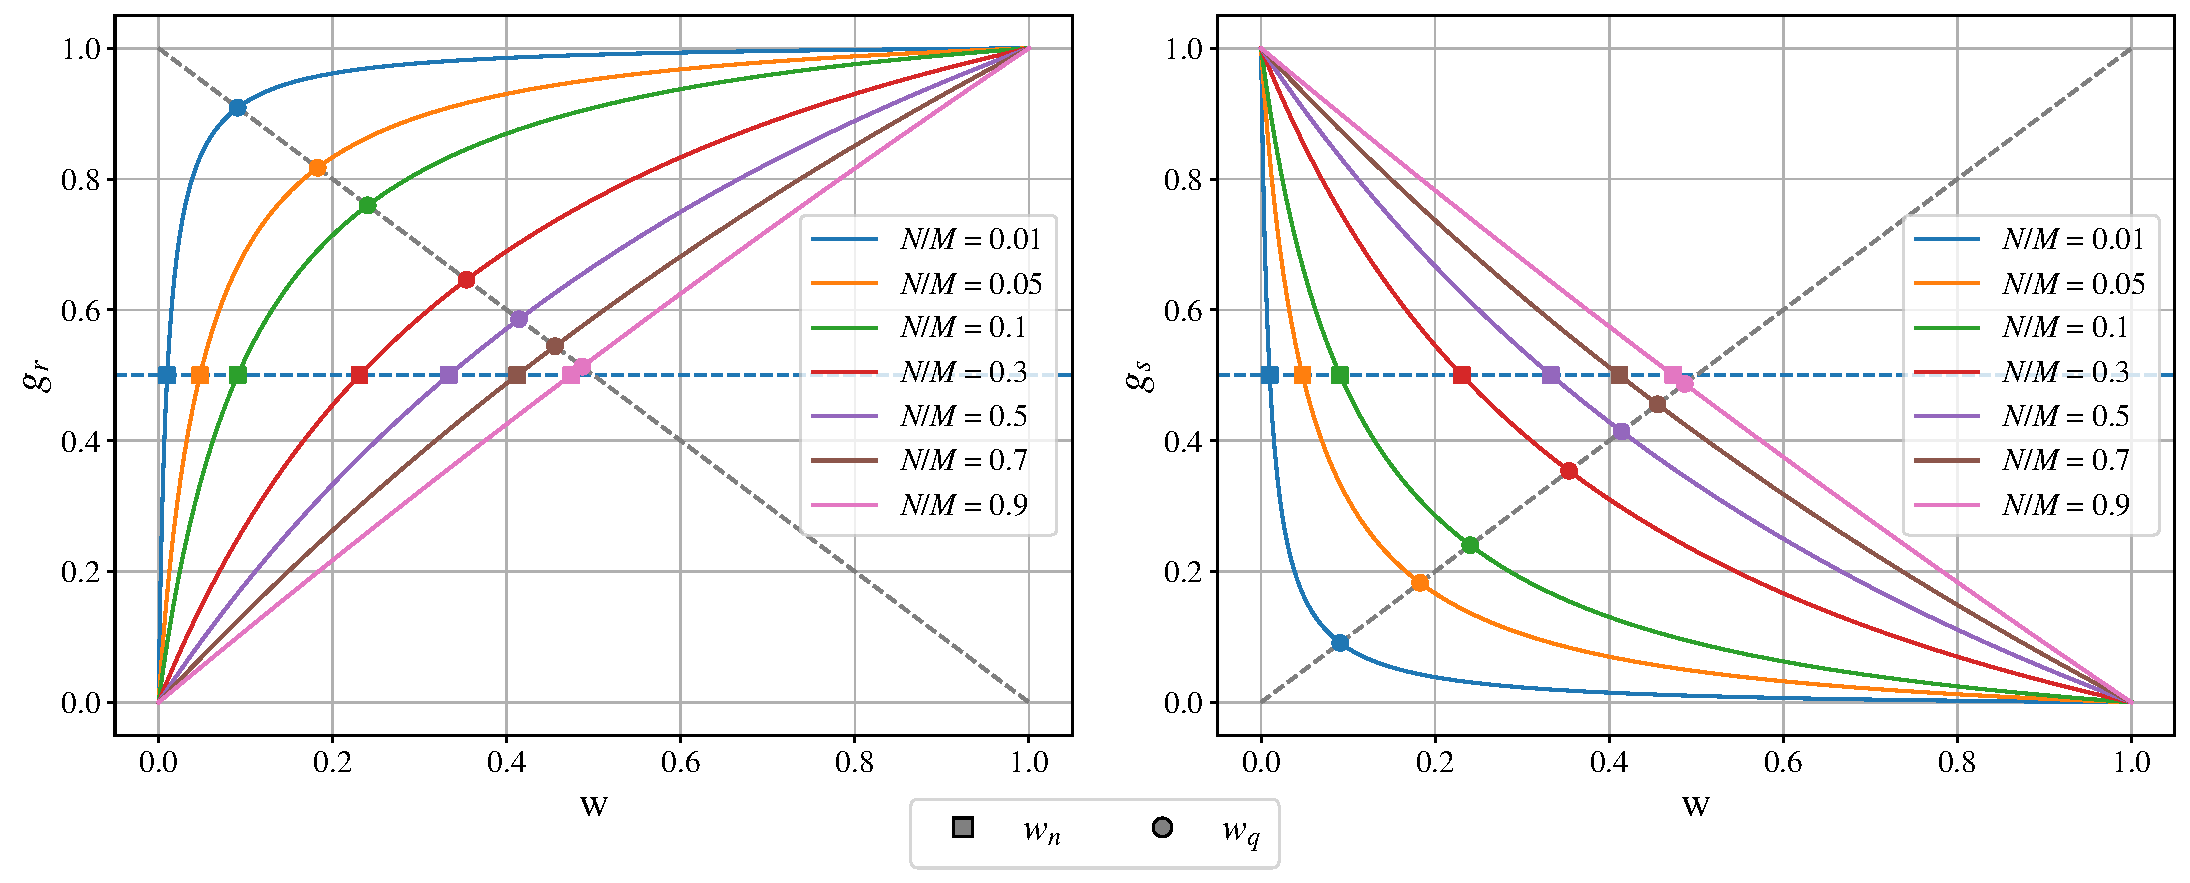
\includegraphics[width=0.95\linewidth]{asset/scaling_factors.pdf}
    \caption{N/M scaling}
    \label{fig:w_scaling}
\end{figure*}

\begin{figure*}[htbp]
    \centering
    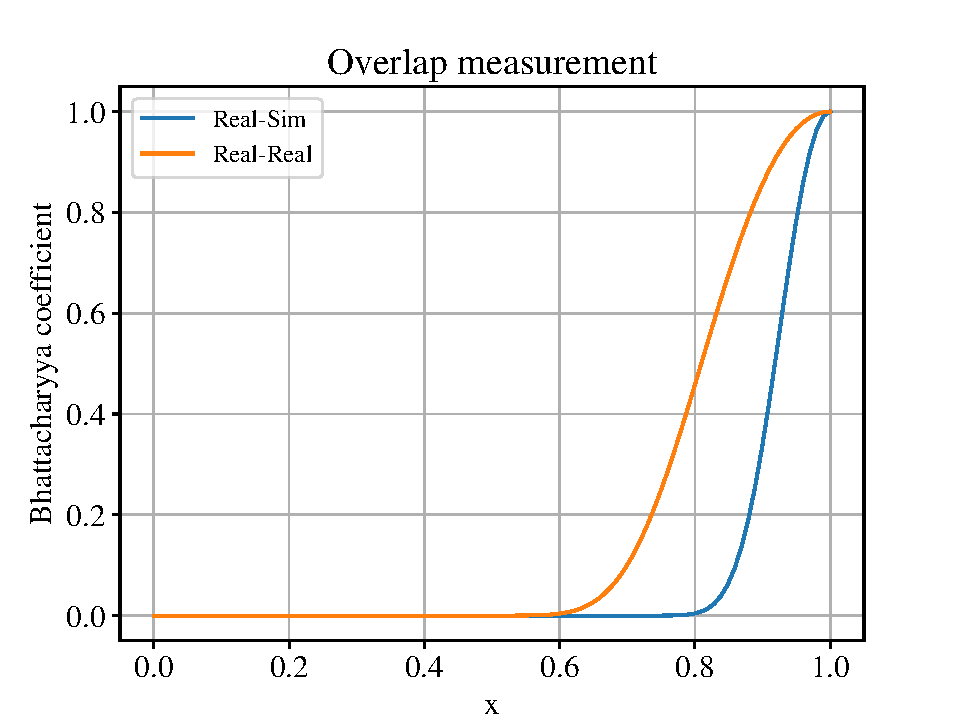
\includegraphics[width=0.5\linewidth]{asset/overlap_measurement.pdf}
    \caption{Empirical measurement about training sample overlapping using Bhattacharyya coefficient. We compute it in the same way as in \citet{song2025selective}, but include the distances between observation features as we are modeling the conditional distribution.}
    % \vspace{-2em}
    \label{fig:overlap measurement}
\end{figure*}

\subsection{Empirical Estimation}
\label{appdx: estimation}
\textbf{[Fact 1. Gaussian concentration in high-dimensional space]:}
for a standard Gaussian vector $\epsilon \sim \mathcal{N}(\mathbf{0}, \mathbf{I}_d)$, we have $||\epsilon|| = \sqrt{d}(1+\mathcal{O}(1))$ with high probability.
So for each component in $p_r(x_t), p_s(x_t)$, it concentrates on a set of thin spherical shells centered at $\alpha_tx_i$ with radius $\sigma_t\sqrt{d}$.

\textbf{[Empirical evidence 1. Data points separation]:}
for most of the timesteps $t$ that are not too large, in high-dimensional data space,
these shells are non-overlapping as $\sigma_t\sqrt{d} \ll \min_{i,j} ||\alpha_t x_i - \alpha_t x_j||$.
We show this in the action-chunking space of diffusion policy as shown in Fig.~\ref{fig:overlap measurement}.

These make the softmax weights extremely imbalanced, which is nearly biased towards the nearest training data.

\textbf{[A Special Case Study]}: Let's assume an ideal case where the action chunks are uniformly distributed across different states on the trajectories, so the ratio of the number of trajectories between simulation and real is similar to the ratio of the number of action chunks of different states between simulation and real.  A special case is that the nearest data points in $\mathcal{D}_r$ are similarly close to the nearest data points in $\mathcal{D}_s$, then we can have:
\begin{equation}
\small
\begin{aligned}
    s_w^*(a^t, t) \approx \frac{\alpha_t}{\sigma_t^2}\left[ \frac{w/N\cdot \exp(-r_r^2/2)}{w/N\cdot \exp(-r_r^2/2)+(1-w)/M \cdot \exp(-r_s^2/2)}\cdot x_r  + \frac{(1-w)/M \cdot \exp(-r_s^2/2)}{w/N\cdot \exp(-r_r^2/2)+(1-w)/M\cdot \exp(-r_s^2)}\cdot x_s \right]
\end{aligned}
\end{equation}

Then we have $\frac{g_r}{g_s} = \frac{1-w_N}{w_N}\cdot \frac{w}{1-w} \cdot \exp(\frac{r_s^2 - r_r^2}{2}) = \frac{1-w_N}{w_N}\cdot \frac{w}{1-w} \cdot \exp (\frac{|a_t - (a_r+a_s)/2|\cdot|a_r-a_s|}{2\sigma_t^2d})$, also we can draw the relation between $g_r,g_s$ and $w$. We can find that as the ratio of sim/real increases, the choice of $w$ should be more robust, which aligns with prior observations from~\citet{wei2025empirical}. And $g_r(w_n)=g_s(w_n)=1/2$, which aligns with our intuition.

Since we find that the curve will be extremely steep for small $N/M$, we posit that the balanced mixing ratio should make good use of both real and sim, but place more weight on real. 
Take the intersection point between $g_r, g_s$ with diagonal $g=1-w$ and $g=w$ , the coordinate of intersection point in $g_r$ is $(w_q, 1-w_q)$ where $w_q=\frac{\sqrt{q}}{\sqrt{q}+1}$ and $q=\frac{N}{M}$.
So the relative domain weight $\frac{g_r}{g_s}$ should be between $(1, \sqrt{\frac{M}{N}})$,
and balanced mixing ratio should be between $(w_n, w_q\approx\sqrt{\frac{N}{M}})$ when $N\gg M$.
With this principle, this range is around $(0.016, 0.13)$ in our experiments which also aligns with our experimental observations.


\section{Training Details}
\label{appdx: training details}

The original images are captured by the camera at a resolution of 720$\times$1280. During
preprocessing, the images are downsampled to 90$\times$106, followed by random cropping to 84$\times$84
during training and center cropping during testing. The policy takes stacked history images and robot
proprioceptive inputs (joint and gripper positions) as input, and outputs 7-DOF target joint positions
along with the gripper action.

The overall training procedure of \textit{CFG-ADDA} is summarized in Algo.~\ref{algo: ours}.
We implement the discriminator as a simple 3-layer MLP.
Across all of our experiments, we use a batch size of 256, dropping probability $p=0.2$ and a weighting coefficient $\lambda=0.1$.
To ensure the discriminator can learn in a compact feature space and also provide effective reverse gradients to the policy, we only start to train the discriminator and compute the discriminative loss after a warming step of 5000.

The implementation of \textit{CFG} and \textit{ADDA} can be seen as only keeping the corresponding computation part in Algo.~\ref{algo: ours}.

\begin{algorithm}[htb]
   \caption{: CFG-ADDA}
   \label{algo: ours}
\begin{algorithmic}[1]
   \STATE {\bfseries Input:} Source dataset $\mathcal{D}_s$, target dataset $\mathcal{D}_t$, mixing ratio $w$, randomly initialized $f_\phi, \pi_\theta$ and discriminator $Disc_\mu$.
   \FOR{iterations $t=1$ to T}
        \STATE Sample data $\{(o_{i_t},a_{i_t})\}$ with size $N\cdot w$ from $\mathcal{D}_t$ and $\{(o_{i_s},a_{i_s})\}$ with size $N\cdot(1-w)$ from $\mathcal{D}_s$
        \STATE Create one-hot embeddings as environment labels $\{c\}=\{c_{i_t}\}\cup\{c_{i_s}\}$
        \STATE Randomly set environment labels as $\varnothing$ with probability $p$
        \STATE Compute features $z_i = f_\phi(o_i)$
        \STATE Compute discriminator loss $\mathcal{L}_{disc}=-\mathbb{E}_{z_i}[\log Disc_\mu(z_{i_s})] - \mathbb{E}_{z_i}[\log(1- Disc_\mu(z_{i_t}))]$
        \STATE Simply concatenate $z_i$ and $c_i$, compute behavior cloning loss $\mathcal{L}_w(z_i, c_i, a_i)$
        \STATE Update $f_\phi, \pi_\theta,Disc_\mu$ with gradient of $\mathcal{L}_w(\phi, \theta) + \lambda \cdot \mathcal{L}_{disc}(\mu)$
   \ENDFOR
\end{algorithmic}
\end{algorithm}



\section{Additional Experiments Results}

\begin{figure*}[tbp]
    \centering
    \begin{subfigure}[t]{0.33\linewidth}
        \centering
        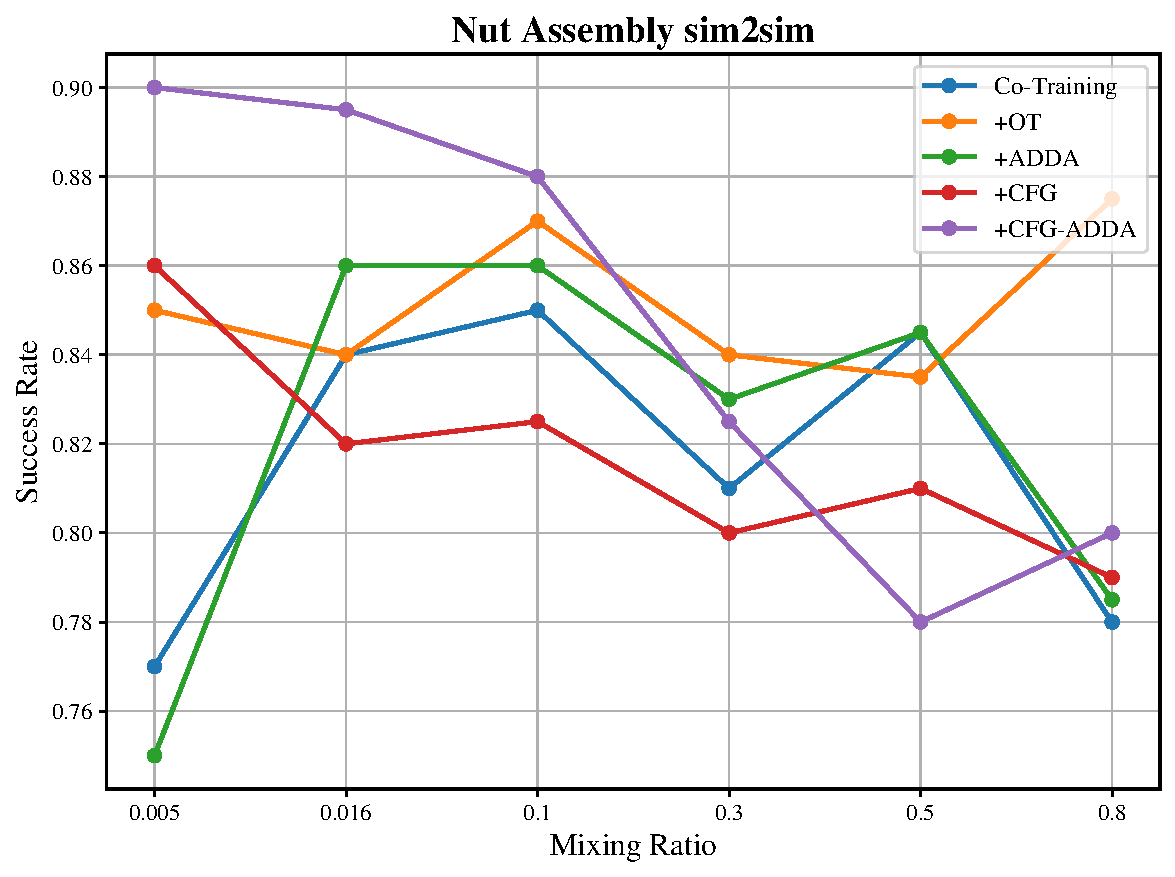
\includegraphics[width=\linewidth]{asset/nutassembly_sim2sim_bench.pdf}
        \caption{\texttt{NutAssembly}}
    \end{subfigure}
    \hfill
    \begin{subfigure}[t]{0.33\linewidth}
        \centering
        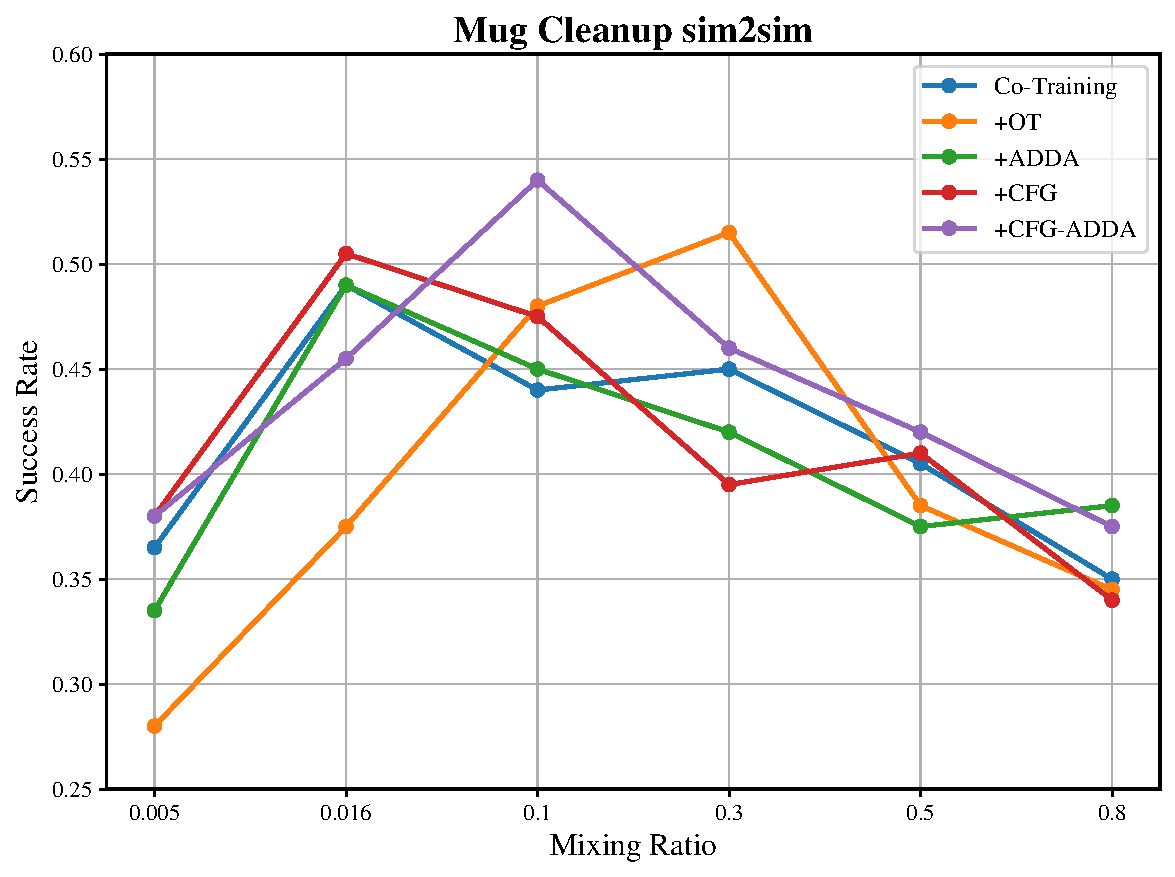
\includegraphics[width=\linewidth]{asset/mugcleanup_sim2sim_bench.pdf}
        \caption{\texttt{MugCleanup}}
    \end{subfigure}
    \hfill
    \begin{subfigure}[t]{0.33\linewidth}
        \centering
        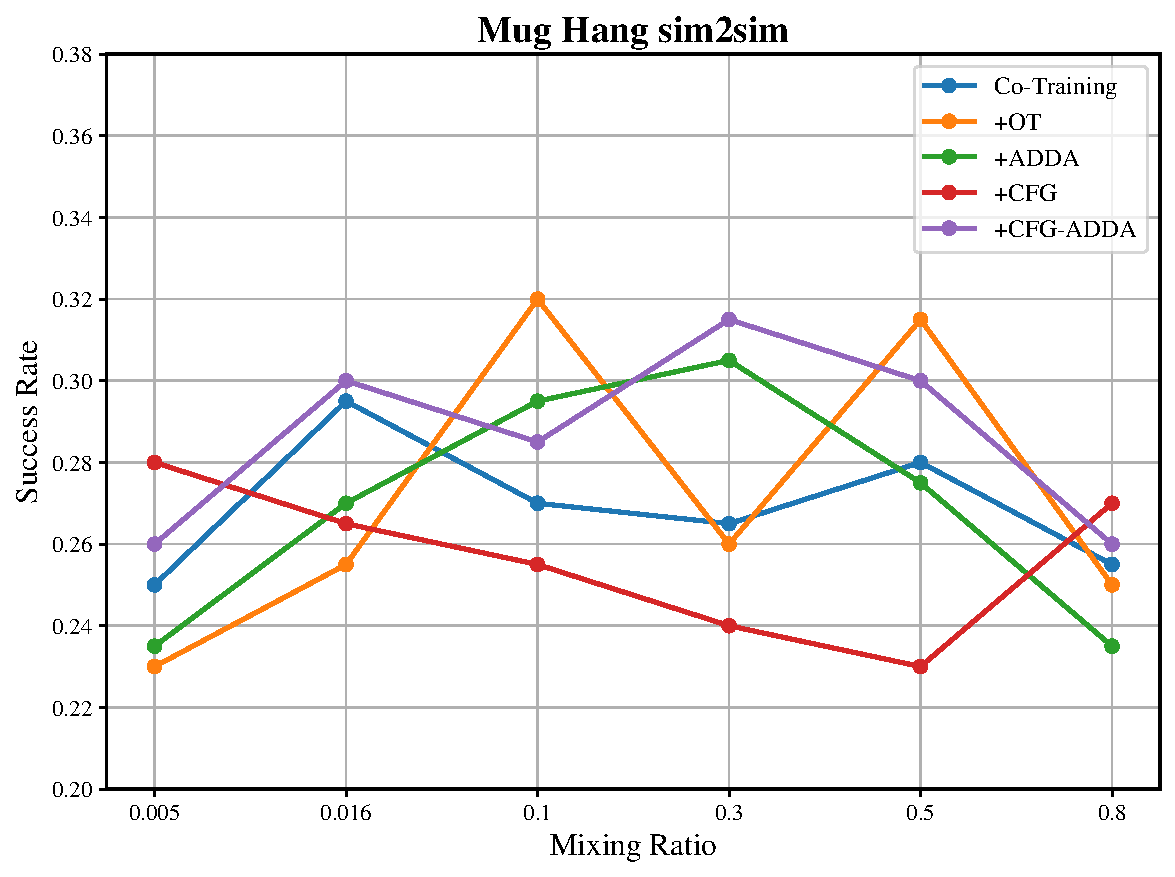
\includegraphics[width=\linewidth]{asset/mughang_sim2sim_bench.pdf}
        \caption{\texttt{MugHang}}
    \end{subfigure}
    % \vspace{-10pt}
    \caption{\textbf{Detailed results of sim-and-sim evaluations.}}
    % \vspace{-20pt}
\end{figure*}


\subsection{Detailed Results of Sim-and-sim Evaluation}
\label{appdx: sim2sim detailed results}
We provide the detailed sim-and-sim evaluation results of comparing different co-training techniques.
In Fig.~\ref{fig: sim2sim eval}, we categorize $0.016, 0.1, 0.3$ as balanced mixing ratio while the others as unbalanced mixing ratio.
Compared to the previous techniques which only emphasizes one side of structured representation alignment, our simple combination brings more stable improvement across different mixing ratios.

\subsection{Details on Representation Alignment}
\label{appdx: more feature vis}

% \begin{figure*}[htbp]
%     \centering
%     \includegraphics[width=0.8\linewidth]{example-image-c}
%     \caption{3D toy example sweeping}
%     \label{fig: 3D toy measure}
% \end{figure*}
\paragraph{Details of Measurement.}
We use UMAP dimension reduction for qualitative visualizations, and measure the Gromov-Wasserstein distance~\cite{memoli2011gromov} and the Wasserstein distance~\cite{ruschendorf1985wasserstein} to show local geometric similarity and global distributional distance for quantitative comparison.
We randomly sample a large batch ($1024$) of data from each domain and normalize the features within each domain independently before quantitative measurement. 
We assume the down-sampled distribution can represent the distribution of the complete dataset.
To compare the Gromov-Wasserstein distance across multiple policies, we normalize the cost matrix by the pooled mean of each domain, thereby controlling for differences in value amplitudes. 


\paragraph{More Feature Visualizations.}
As shown in Fig.~\ref{fig: more feature vis}, the changing trends of the two distances with mixing ratios are similar across different tasks.
When $w$ is in the range of balanced mixing ratio (roughly between $w_n$ and $0.5$), 
the representations of simulation and real-world observations share more similar geometric structures and exhibit greater overlap.



\subsection{Robustness to Different Policy Architectures}
\label{appdx: robustness to architecture}

As our main experiments are all conducted on encoder-decoder transformer-based diffusion policy, to further support the robustness of our findings to different architectures, we do another series of experiments with the same setting on two other architectures --- decoder-only transformer-based model and CNN-based U-Net diffusion policy. 
The results in Fig.~\ref{fig: robustness} show that the best performance consistently lies in a narrow range ([0.016, 0.3]), indicating robustness beyond the architecture used in the main paper.

\begin{figure*}[tbp]
\centering
    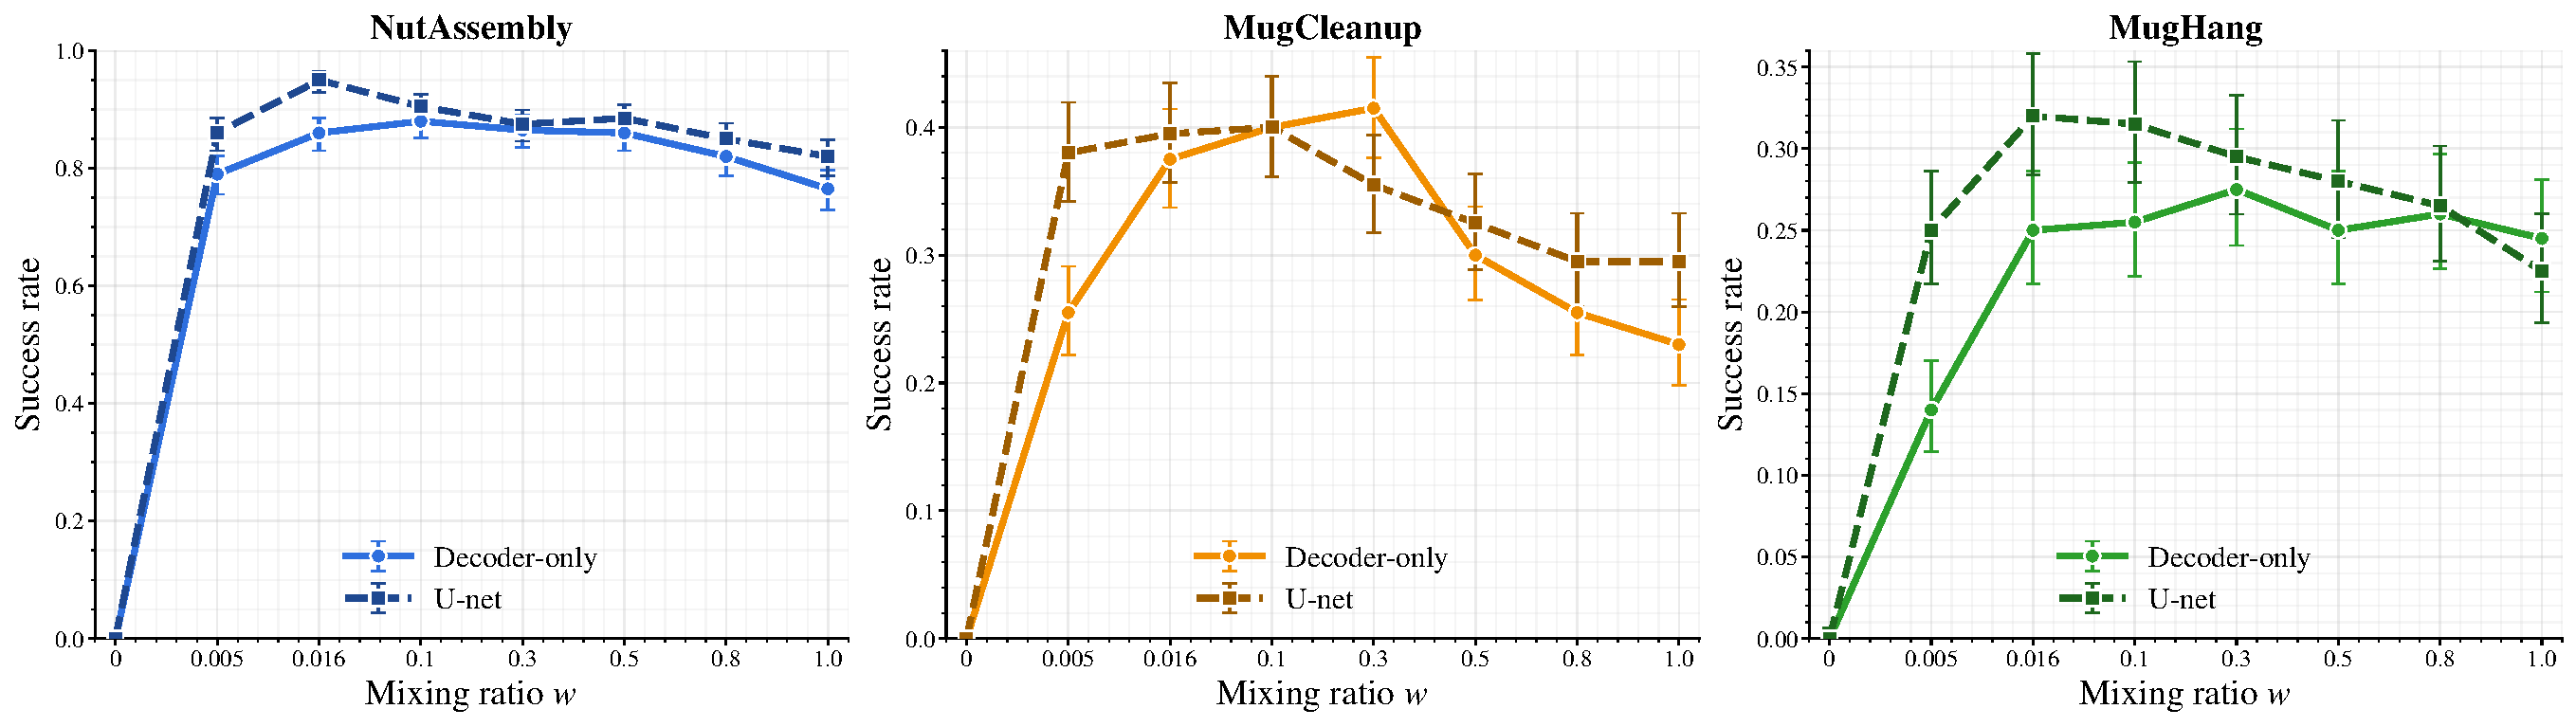
\includegraphics[width=\linewidth]{asset/architecture_robustness.pdf}
    \caption{\textbf{Balanced mixing ratios are robust to different policy architectures.} Each data point is computed over three policy checkpoints, and each checkpoint is evaluated for 200 trials.
    The best performance is consistently achieved in the range of $(0.016, 0.3)$.}
    % We can find that as the domain gaps increase, the model performance usually drops, \textit{e.g.} from visual-only to visual-physics.}
    \label{fig: robustness}
\end{figure*}


\subsection{Comparison to ``Simulation Pre-training+Real Fine-tine"}
\label{appdx: sim pretrain+real finetune}

Although some prior work shows that it is generally less effective than co-training, as this still remains as an important baseline, we include a direct comparison here. 
We pre-train with simulation data only for $\sim130k$ steps and fine-tune with real data for $\sim120k$ steps.
We evaluate all checkpoints along the training and report the highest success rate.
Our result is consistent with prior findings.

\begin{table}[h]
\centering
\small
\begin{tabular}{lcc}
\hline
Task & Pretrain+FT & Co-training \\
\hline
NutAssembly & 0.77  & \textbf{0.925} \\
MugCleanup & 0.215 & \textbf{0.495} \\
MugHang & 0.225 & \textbf{0.26}  \\
\hline
\end{tabular}
\caption{Performance comparison with Pre-train+FT.}
\label{tab: pretrain+ft}
\end{table}

\subsection{A Formal Statement of Mixing Ratio Selection Guideline}
\label{appdx: guideline}

The main experiments in the paper rely a heuristic defined mixing ratio grids. Based on the above analysis, we provide a guideline for selecting mixing ratios for co-training, which we hope will be useful to the community. 
We conduct some additional experiments to further support the effectiveness of our guideline.
We co-train with 3 sets of different dataset sizes -- 10:3000, 50:500, and 50:100 -- and sweep the mixing ratios.

\begin{figure*}[htb]
\centering
    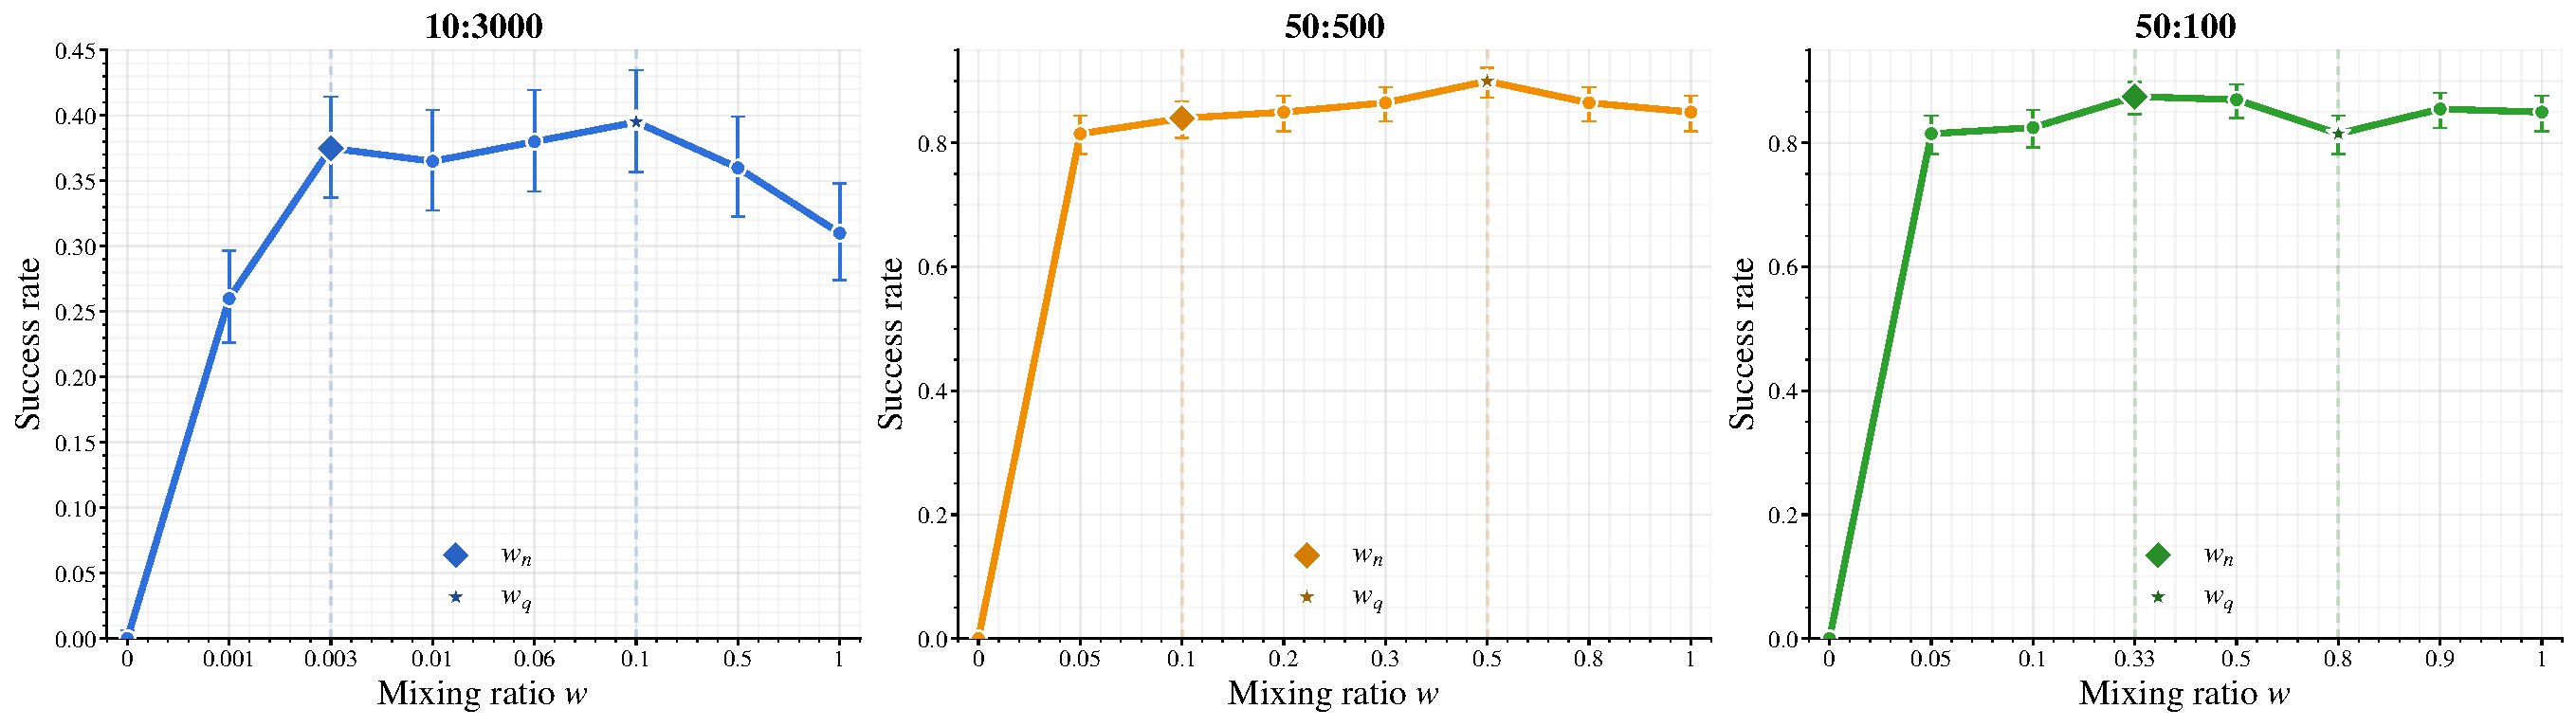
\includegraphics[width=\linewidth]{asset/dataset_ratios.pdf}
    \caption{\textbf{Experiments on different dataset sizes.} Each data point is computed over three policy checkpoints, and each checkpoint is evaluated for 200 trials.
    The best performance is consistently achieved in the range of $(w_n, w_q)$, which supports our guideline below.}
    % We can find that as the domain gaps increase, the model performance usually drops, \textit{e.g.} from visual-only to visual-physics.}
    \label{fig: dataset ratio}
\end{figure*}



\begin{algorithm}[t]
\caption{Guideline for Co-Training Mixing Ratio Selection}
\label{alg: selection}
\begin{algorithmic}[1]
\REQUIRE Source dataset size $N$, target dataset size $M$ with $M > N$
\REQUIRE Optional desired target contribution $q$ (e.g., $q=0.8$)
\ENSURE A narrowed search range $(w_n, w_q)$ for the mixing ratio

\STATE Compute the natural mixing ratio
\[
w_n = \frac{N}{N+M}.
\]
\STATE Use $w_n$ as the lower bound of the search range.

\IF{$M/N > 5$}
    \STATE Set the upper bound as
    \[
    w_q = \sqrt{\frac{N}{M}}.
    \]
\ELSE
    \STATE Set a desired target contribution ratio $q$ (e.g., $q=0.8$).
    \STATE Compute the upper bound as
    \[
    w_q = \frac{N*q}{(1-q)*M + N*q}.
    \]
    \STATE Optionally, set the upper bound empirically to $0.5$, which is empirically enough.
\ENDIF

\STATE Adjust $w_n,w_q$ upward if the source-target domain gap is large.
\STATE Consider domain gaps from visual appearance, physics, and embodiment.
\STATE Since no formal estimator is assumed, apply this adjustment accordingly.

\STATE Perform a simple search for the final mixing ratio within
\[
(w_n,\, w_q).
\]

\end{algorithmic}
\end{algorithm}


\subsection{Three Regimes of ``Representation" in Co-Training}
\label{appdx: three regime}

In Sec.~\ref {sec: condition representation} of the main paper, we point out three different hypothetical scenarios of representation in co-training -- overlapping, structured aligned, and disjoint.
As mentioned above, we use two coupled and measurable properties to characterize the concept of ``structured representation alignment". So it can be mathematically defined as follows: $$\mathcal{SRA}(p_s,p_t) = (\mathcal{M}_{align}, \mathcal{D}_{disc})$$
where $\mathcal{M}_{align}=\mathcal{W}(p_s(z),p_t(z))$ and $\mathcal{D}_{\mathrm{disc}} = \frac{1}{2} \sum_{k \in \{s,t\}} \mathbb{E}_{z \sim p_k(z)} \left[ \max_{a^t} p_k(a^t \mid z) \right]$. 
We design another set of experiments to show the existence of these three regimes:
We introduce an additional and complementary control knob via discriminator regularization, which directly modulates domain discernibility. Specifically, we train models with discriminator loss weights of \{0, 0.05, 0.5\}, and within each setting sweep the mixing ratio to vary alignment. This allows us to populate a substantially broader region of the (alignment, discernibility) space.

Empirically, these settings correspond to different regimes:
(1) No discriminator (0): representations remain weakly aligned (high WD) but highly distinguishable (high discernibility), corresponding to the disjoint regime (and partially covering the boundary toward structured alignment).
(2) Moderate discriminator (0.05): representations become better aligned (lower WD) while preserving domain-specific structure (high discernibility), corresponding to the desired structured aligned regime.
(3) Strong discriminator (0.5): representations are strongly aligned (low WD), but domain-specific information is suppressed (low discernibility), corresponding to the overlapping regime.
Within each regime, varying the mixing ratio further modulates the degree of alignment, producing a set of points spanning different Wasserstein distances.

We provide the corresponding 2D visualization (including Wasserstein distance) in Fig.~\ref{fig: three regimes}. We observe:
- In the overlapping regime, the correlation between performance and WD is reversed, consistent with observations in physics-only settings.
- In the disjoint regime, the correlation follows the standard co-training trend (better alignment improves performance).
- In the structured aligned regime, the correlation remains positive but weaker, indicating a distinct intermediate behavior.

Taken together, these regimes exhibit a non-monotonic relationship, resulting in a characteristic \textbf{inverted-U (or U-shaped) curve} when alignment and discernibility are jointly considered. This unifies the three regimes as different regions of a single underlying mechanism.

\begin{figure*}[htbp]
    \centering
    % \captionsetup{font={small}}
    \resizebox{\textwidth}{!}{
    \begin{subfigure}{\linewidth}
        % \centering
        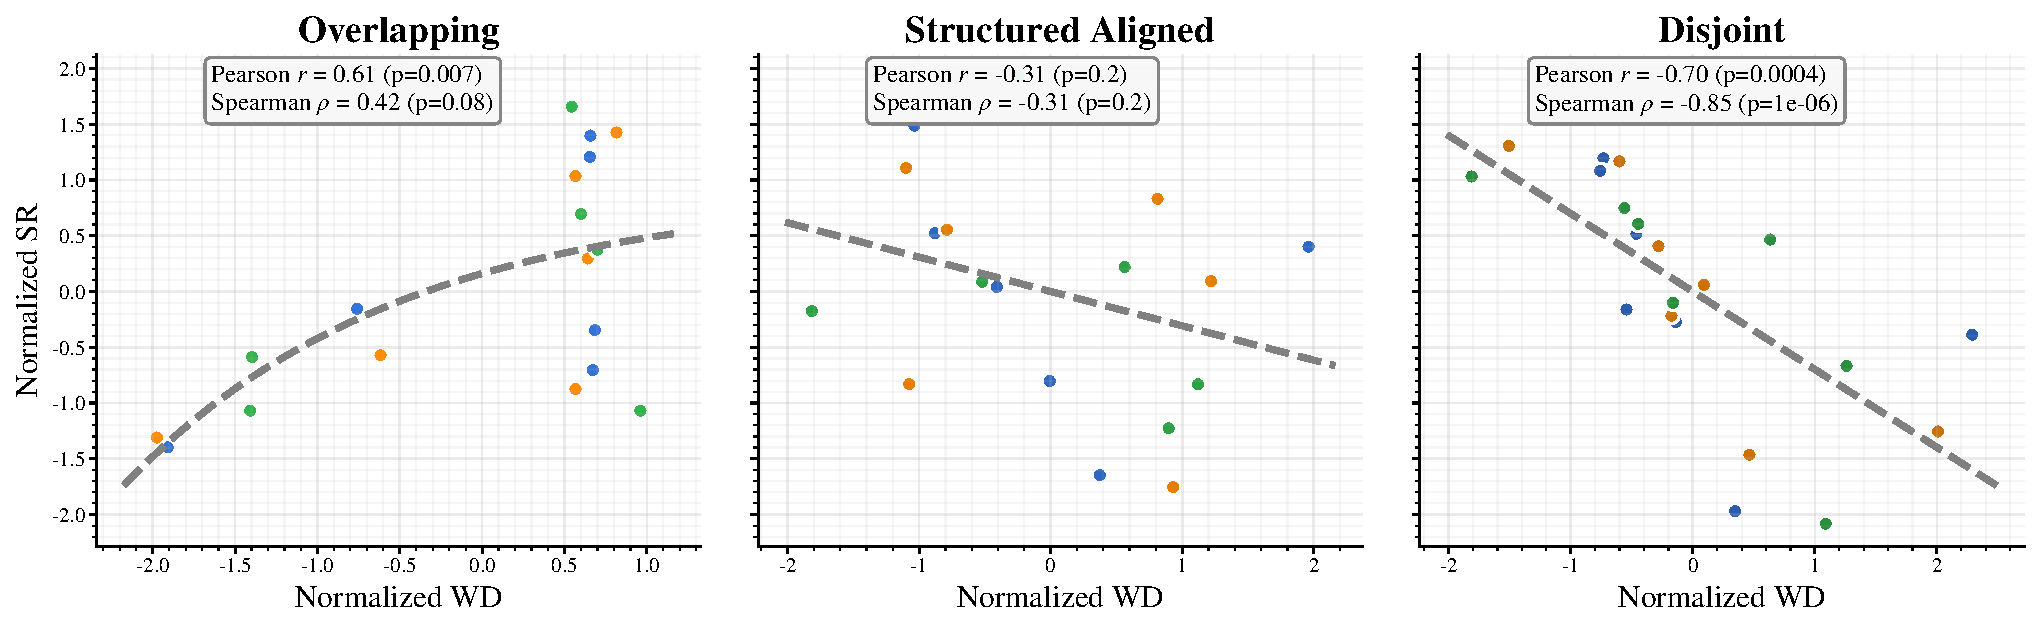
\includegraphics[width=\textwidth]{asset/three_regimes_horizontal.pdf}
        \caption{\textbf{Three regimes exhibit U-shape correlation pattern.}}
        \label{fig: three regimes horizontal}
    \end{subfigure}}
    \vfill
    \resizebox{0.85\textwidth}{!}{
    \begin{subfigure}{\linewidth}
        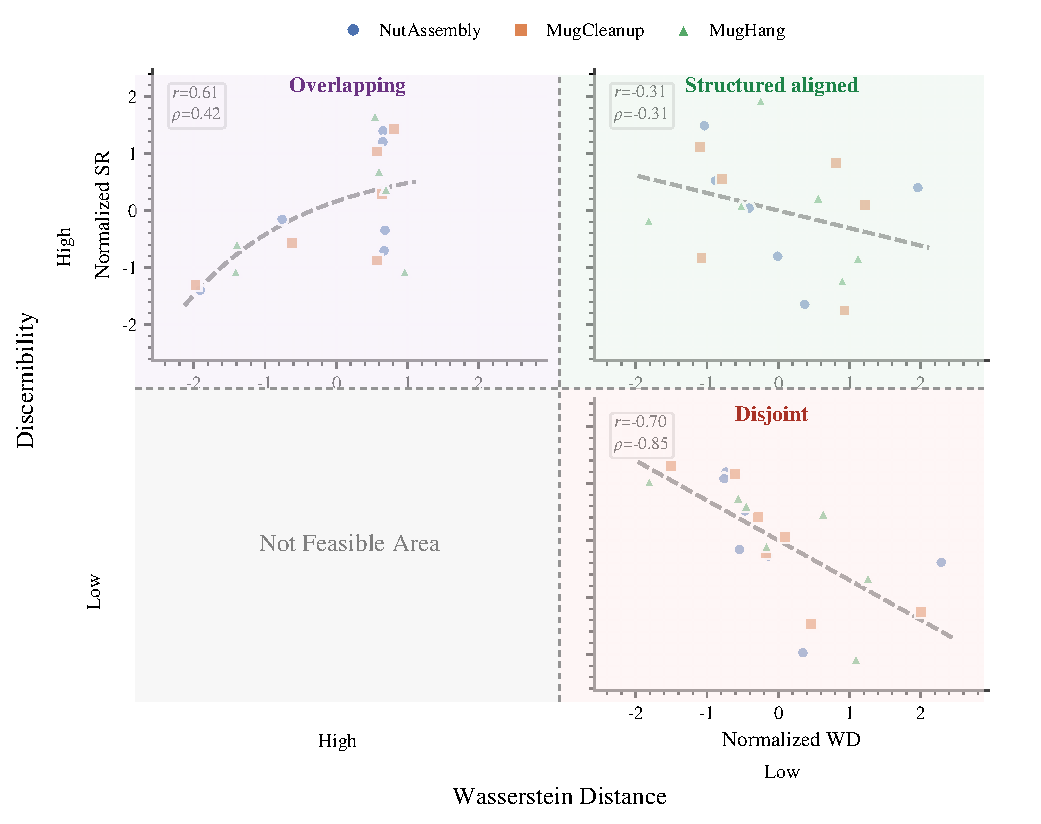
\includegraphics[width=\textwidth]{asset/three_regimes_2x2.pdf}
        \caption{\textbf{Three regimes on two-axises -- representation alignment and domain discernibility.}}
        \label{fig: three regimes 2x2}
    \end{subfigure}}
    % \vspace{-0.5em}
    \caption{\textbf{Existence of three regimes in co-training.}}
    \vspace{-20pt}
    \label{fig: three regimes}
\end{figure*}



\begin{figure}[t]
    \centering
    \captionsetup{font={small}}
    \resizebox{0.98\linewidth}{!}{
    \begin{subfigure}{\linewidth}
        % \centering
        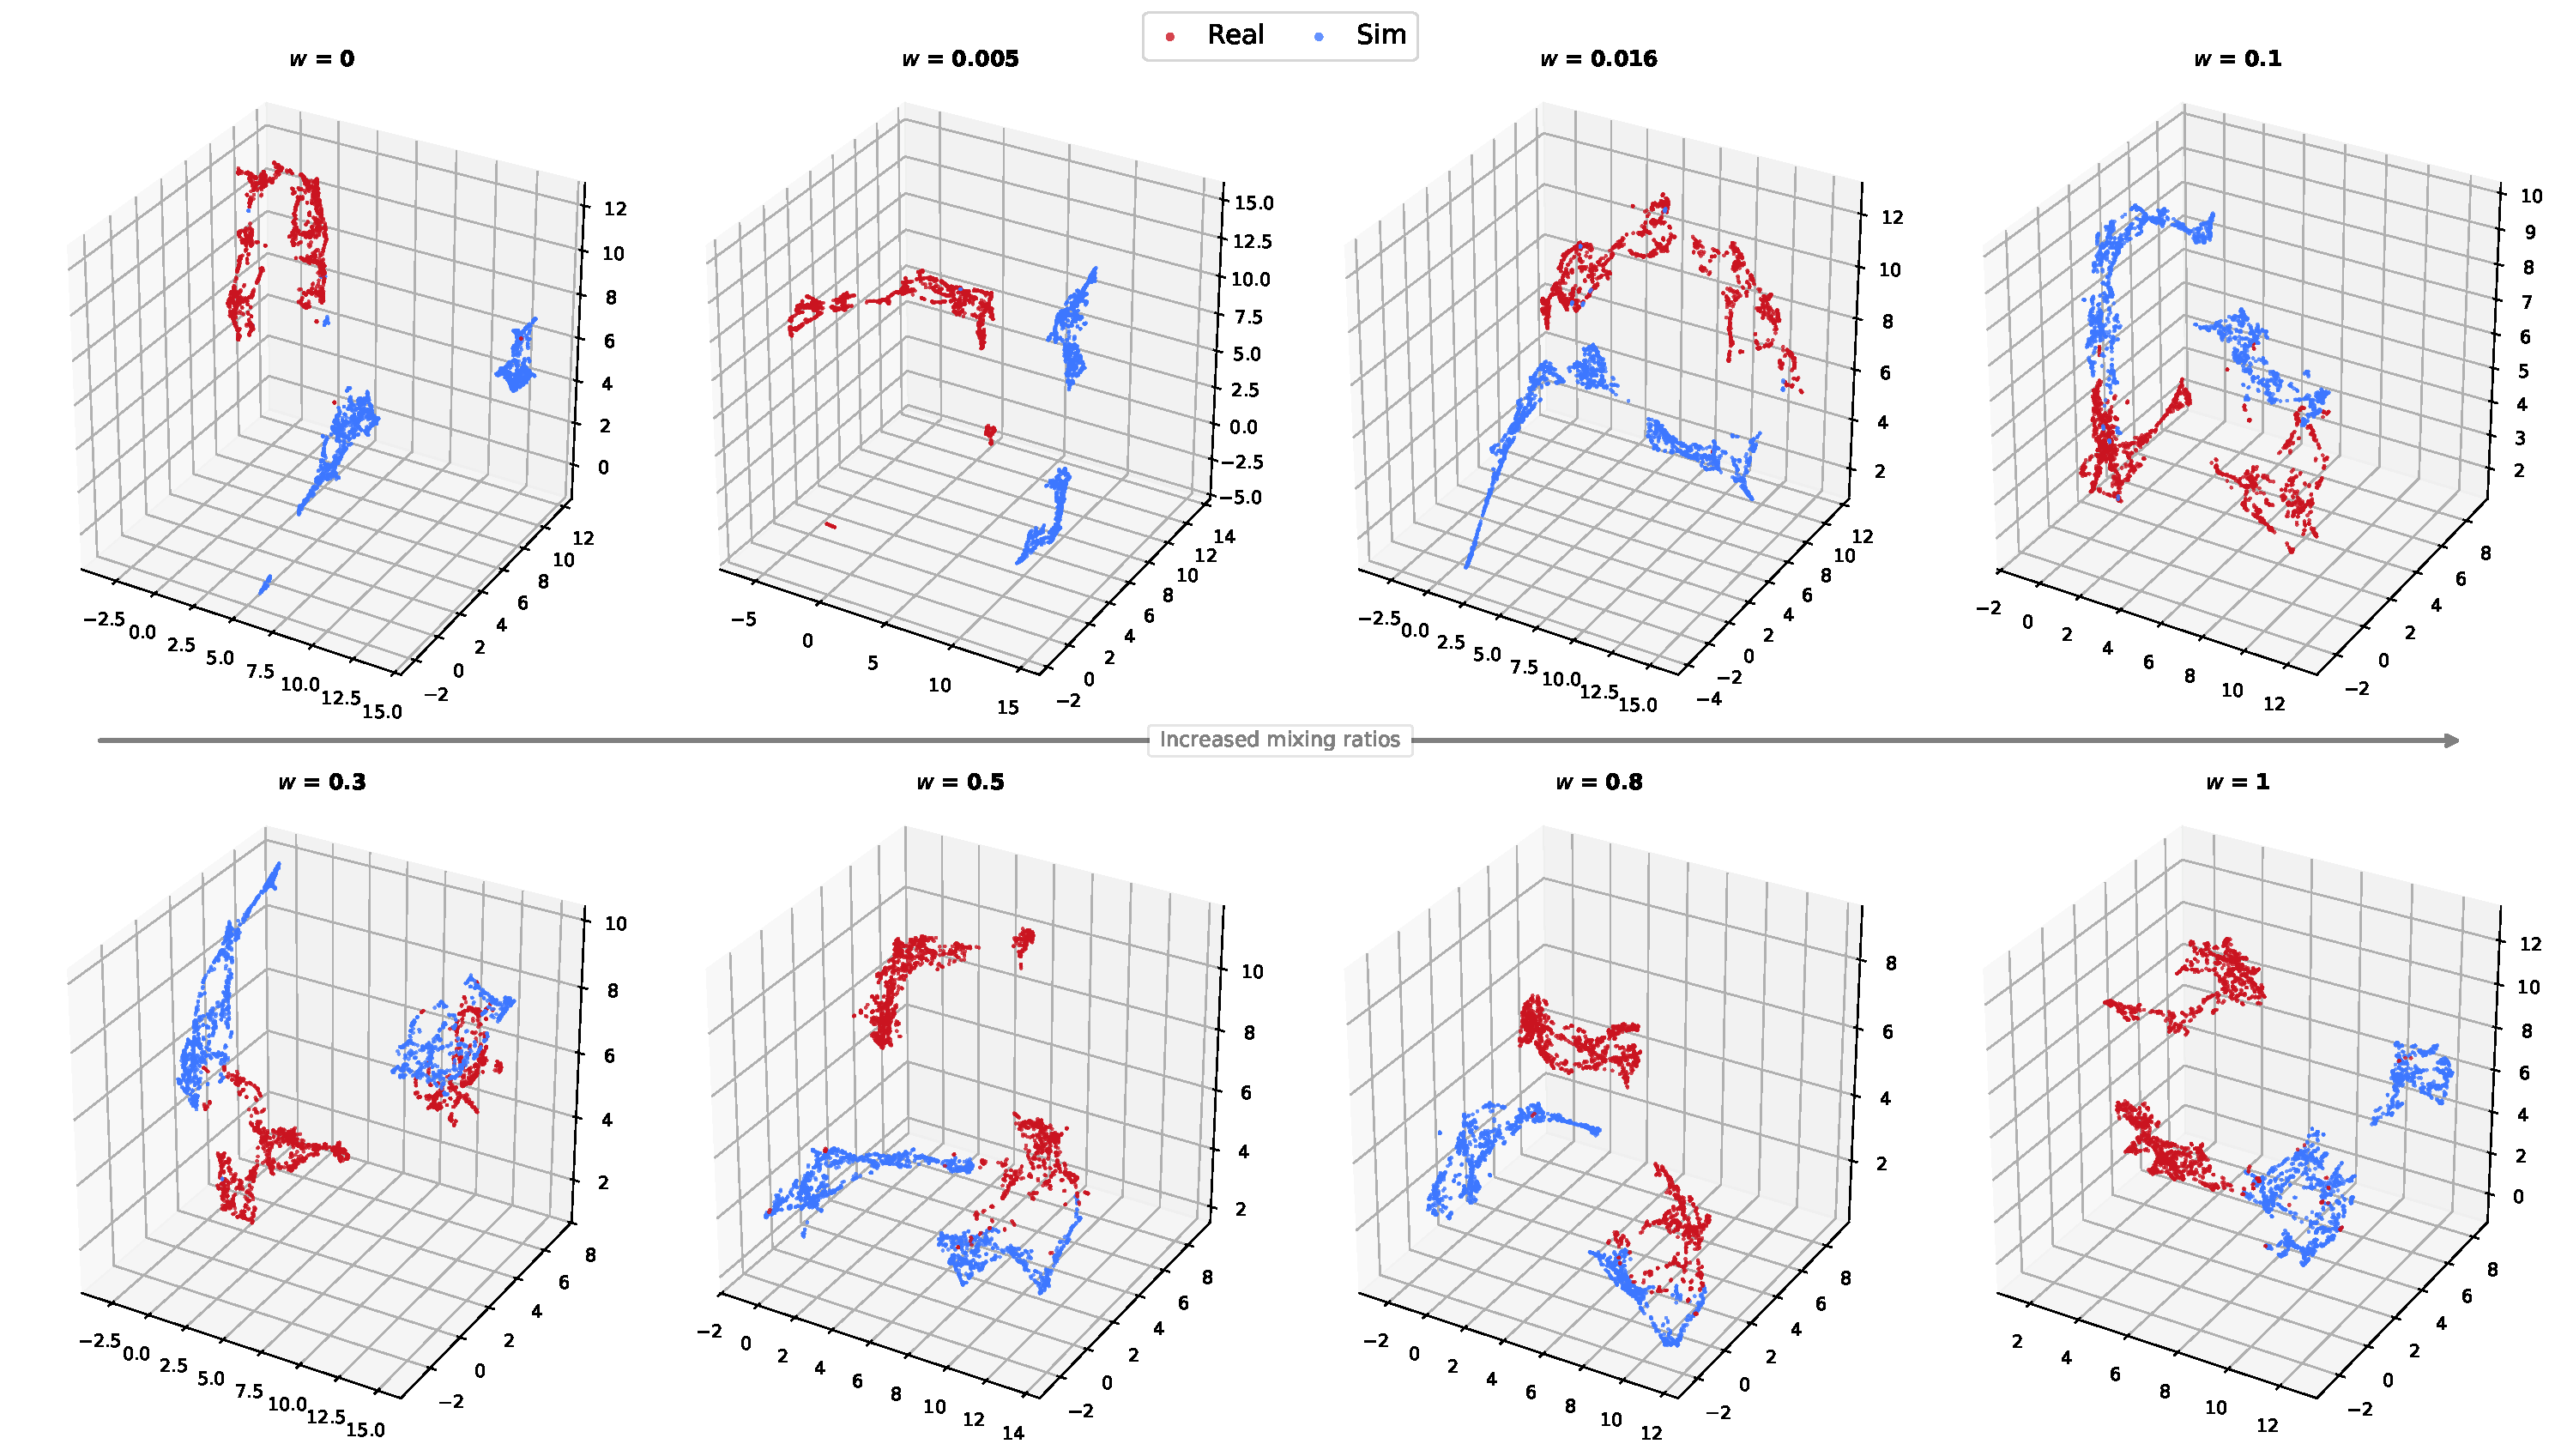
\includegraphics[width=\textwidth, height=2.8in]{asset/nutassembly_img_feat_3d.pdf}
        \caption{\texttt{NutAssembly}.}
    \end{subfigure}}
    \vfill
    \resizebox{0.98\linewidth}{!}{
    \begin{subfigure}{\linewidth}
        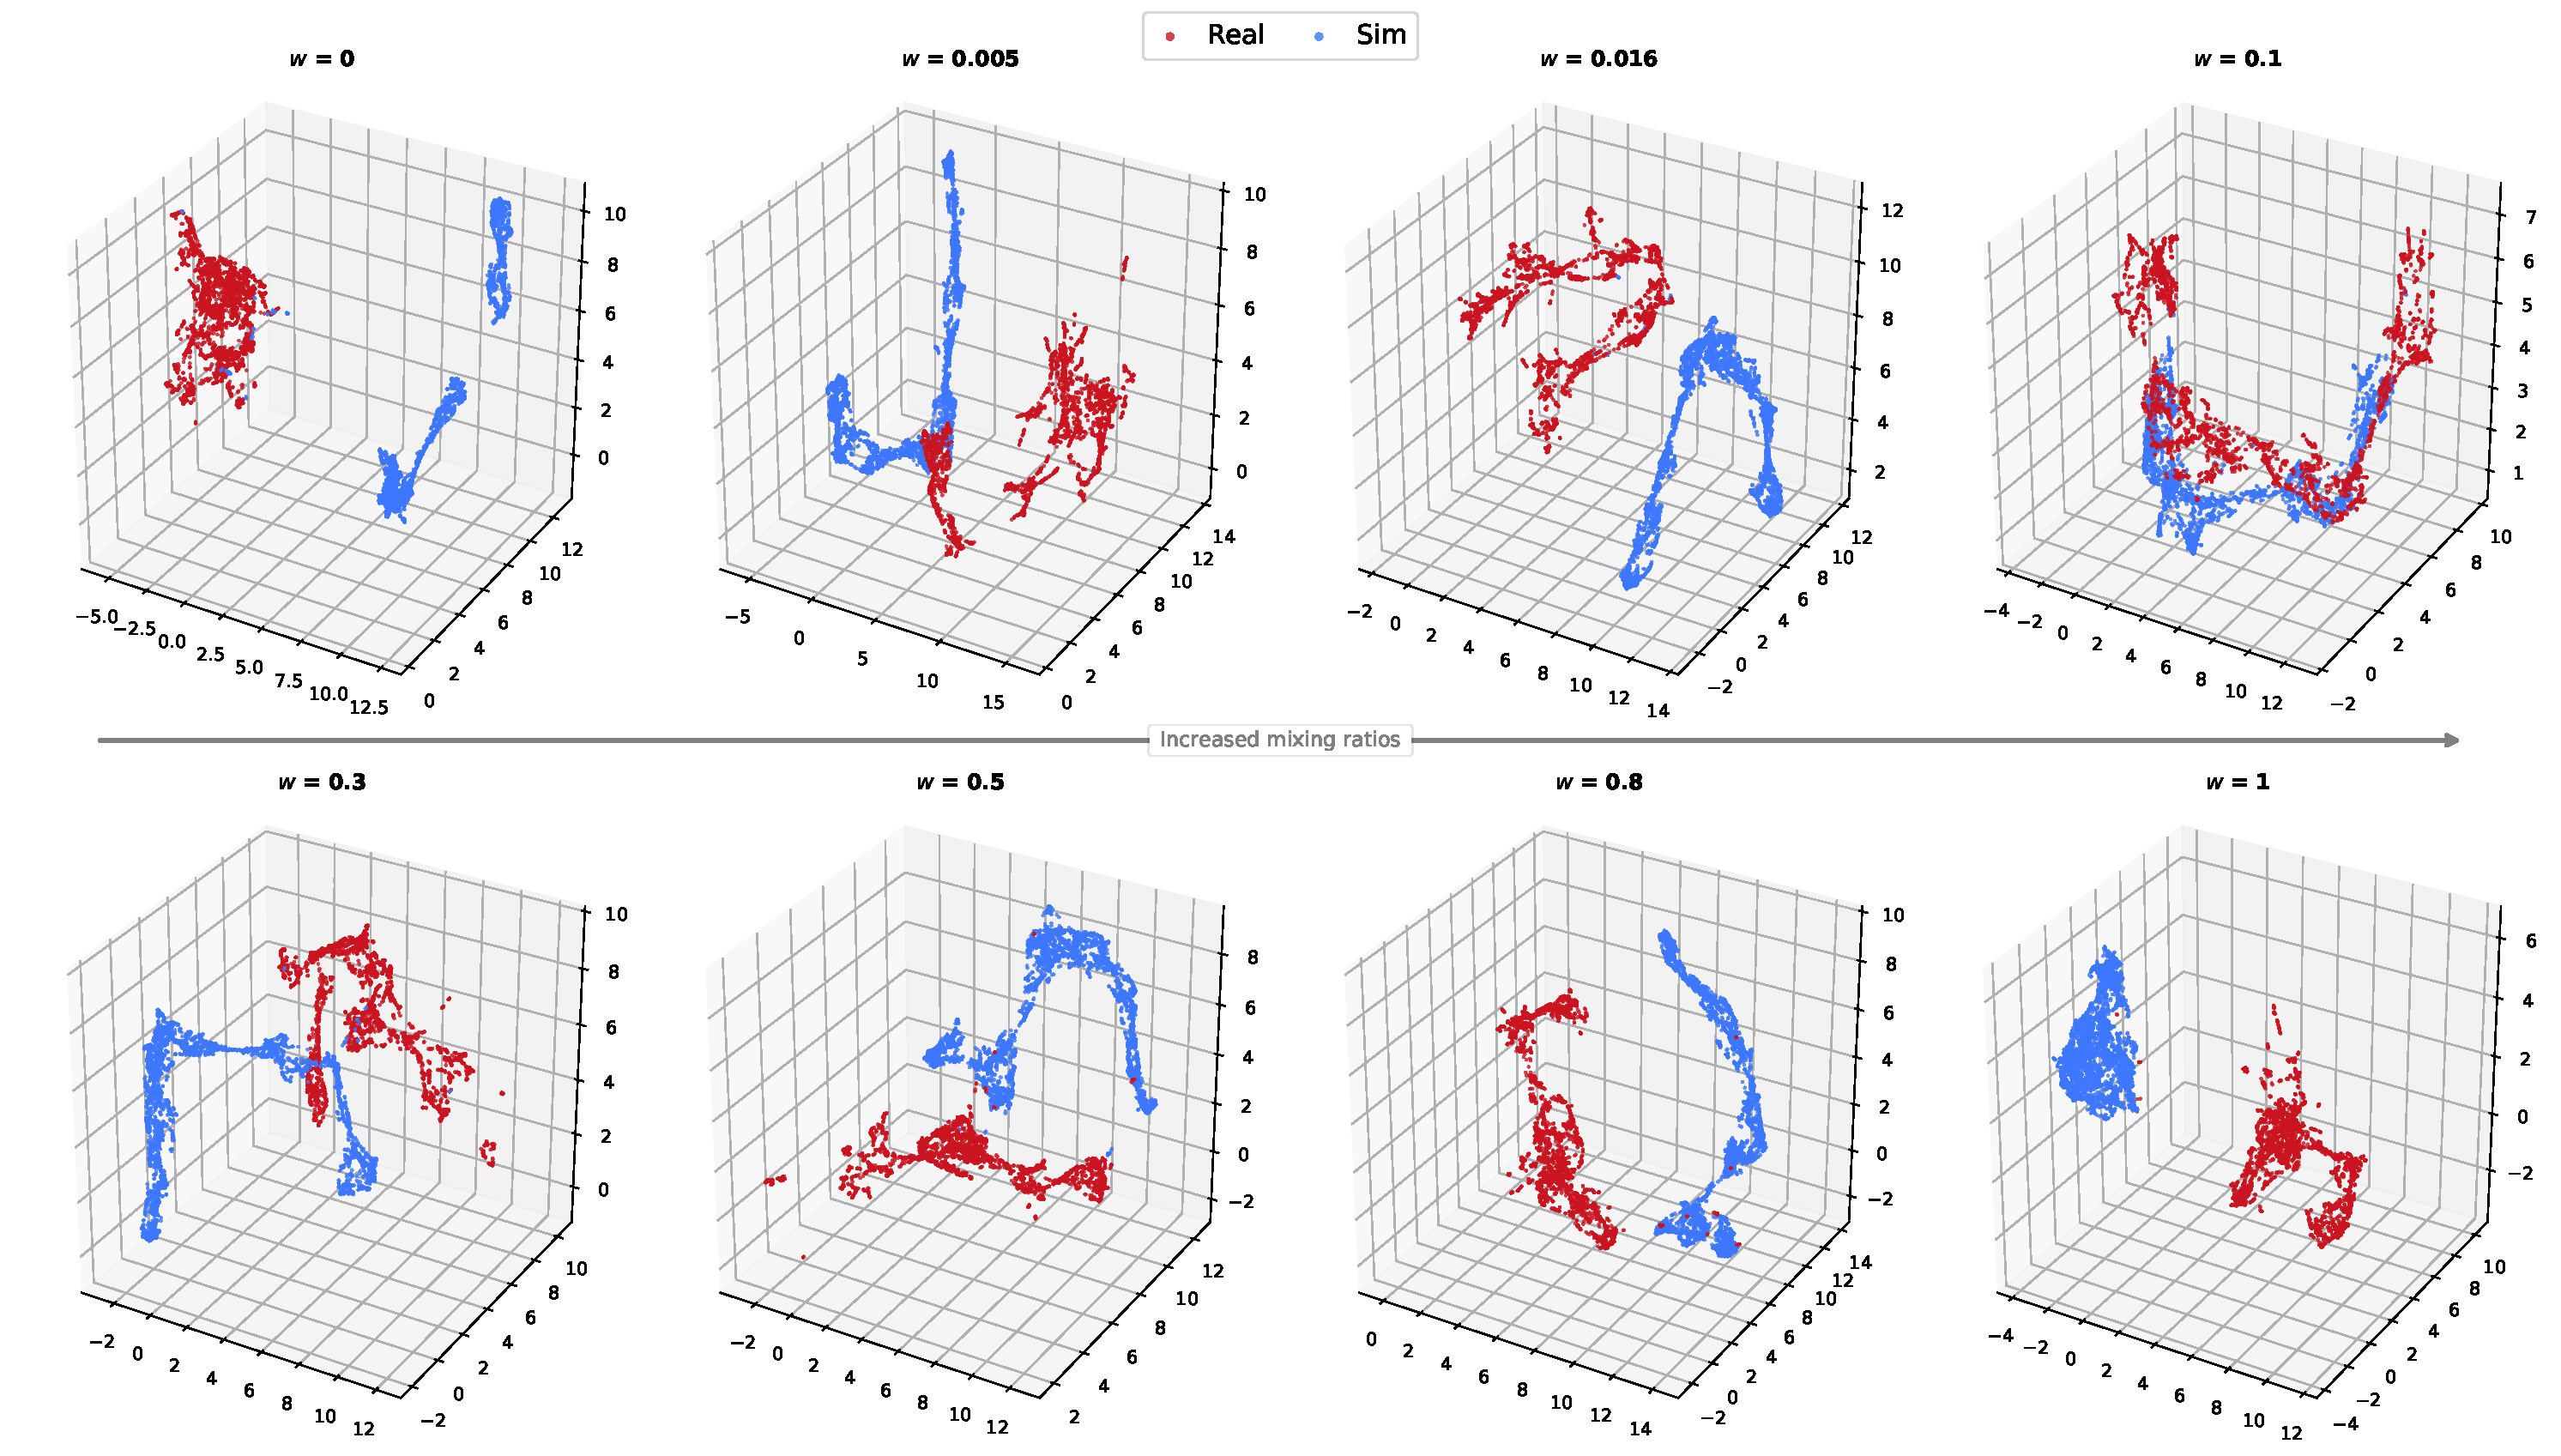
\includegraphics[width=\textwidth, height=2.8in]{asset/mugcleanup_img_feat_3d.pdf}
        \caption{\texttt{MugCleanup}.}
    \end{subfigure}}
    \vfill
    \resizebox{0.98\linewidth}{!}{
    \begin{subfigure}{\linewidth}
        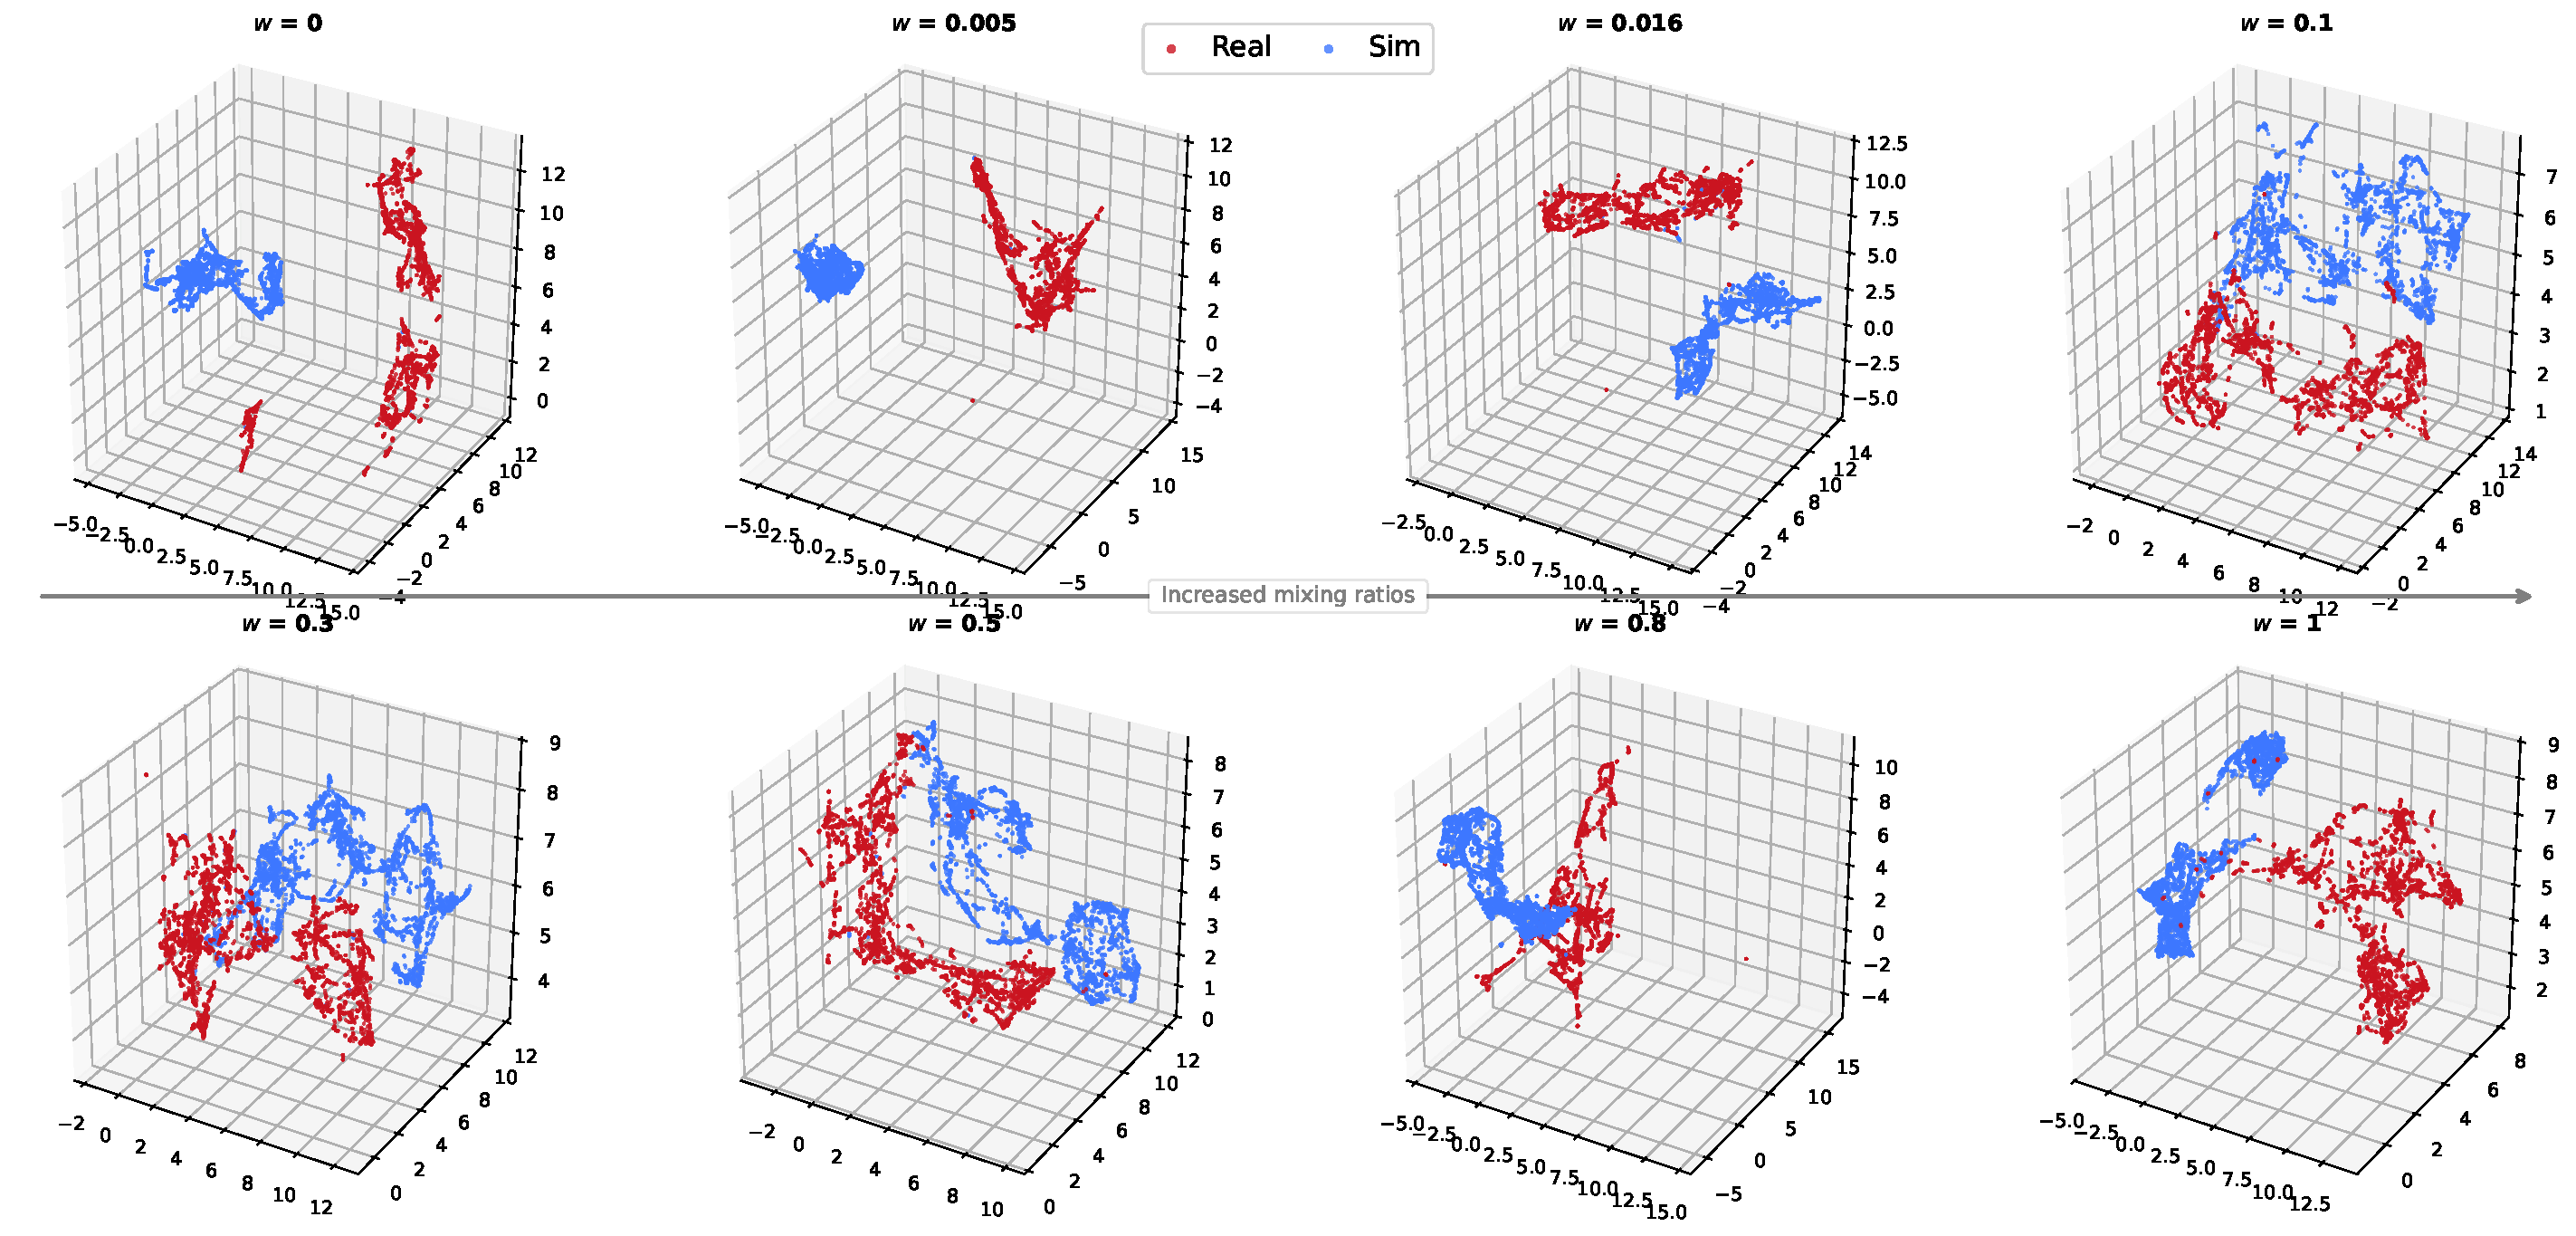
\includegraphics[width=\textwidth, height=2.8in]{asset/mughang_img_feat_3d.pdf}
        \caption{\texttt{MugHang}.}
    \end{subfigure}}
    \caption{\textbf{More UMAP visualizations of the observation representations.} }
    \vspace{-10pt}
    \label{fig: more feature vis}
\end{figure}

\begin{figure}[t]
    \centering
    \captionsetup{font={small}}
    \resizebox{0.98\linewidth}{!}{
    \begin{subfigure}{\linewidth}
        % \centering
        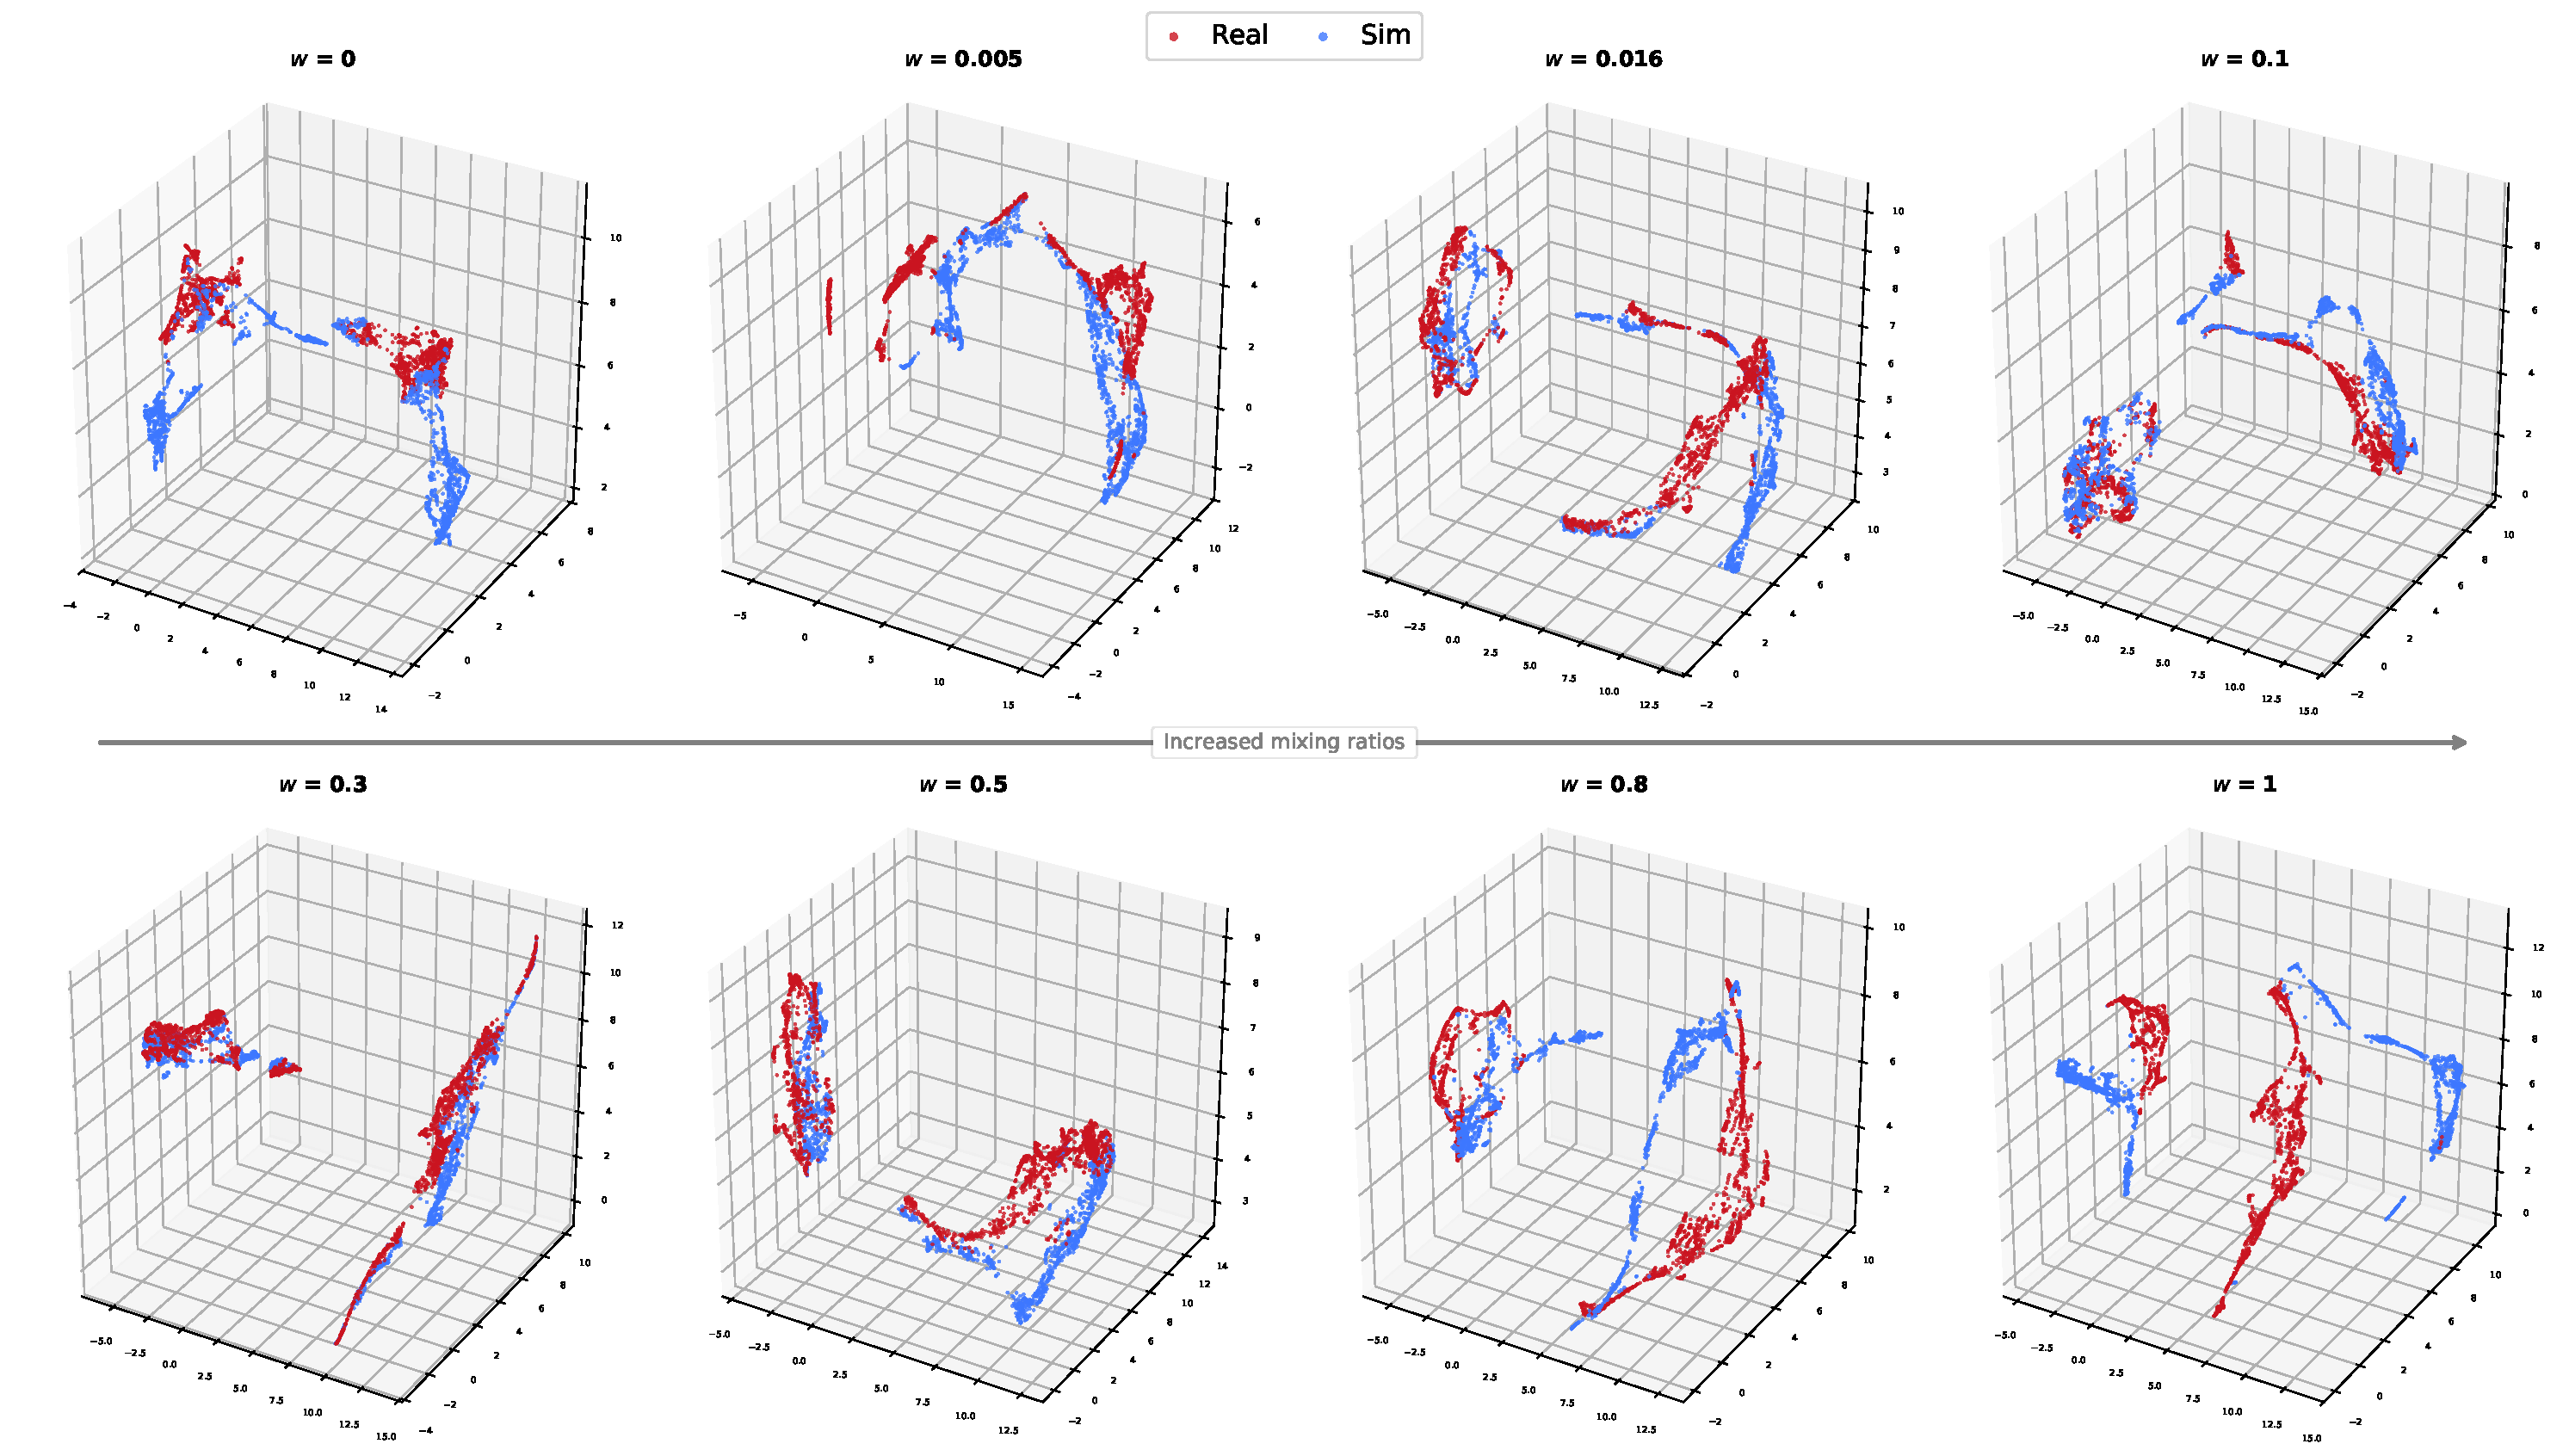
\includegraphics[width=\textwidth, height=2.8in]{asset/nutassembly_trans_feat.pdf}
        \caption{\texttt{NutAssembly}.}
    \end{subfigure}}
    \vfill
    \resizebox{0.98\linewidth}{!}{
    \begin{subfigure}{\linewidth}
        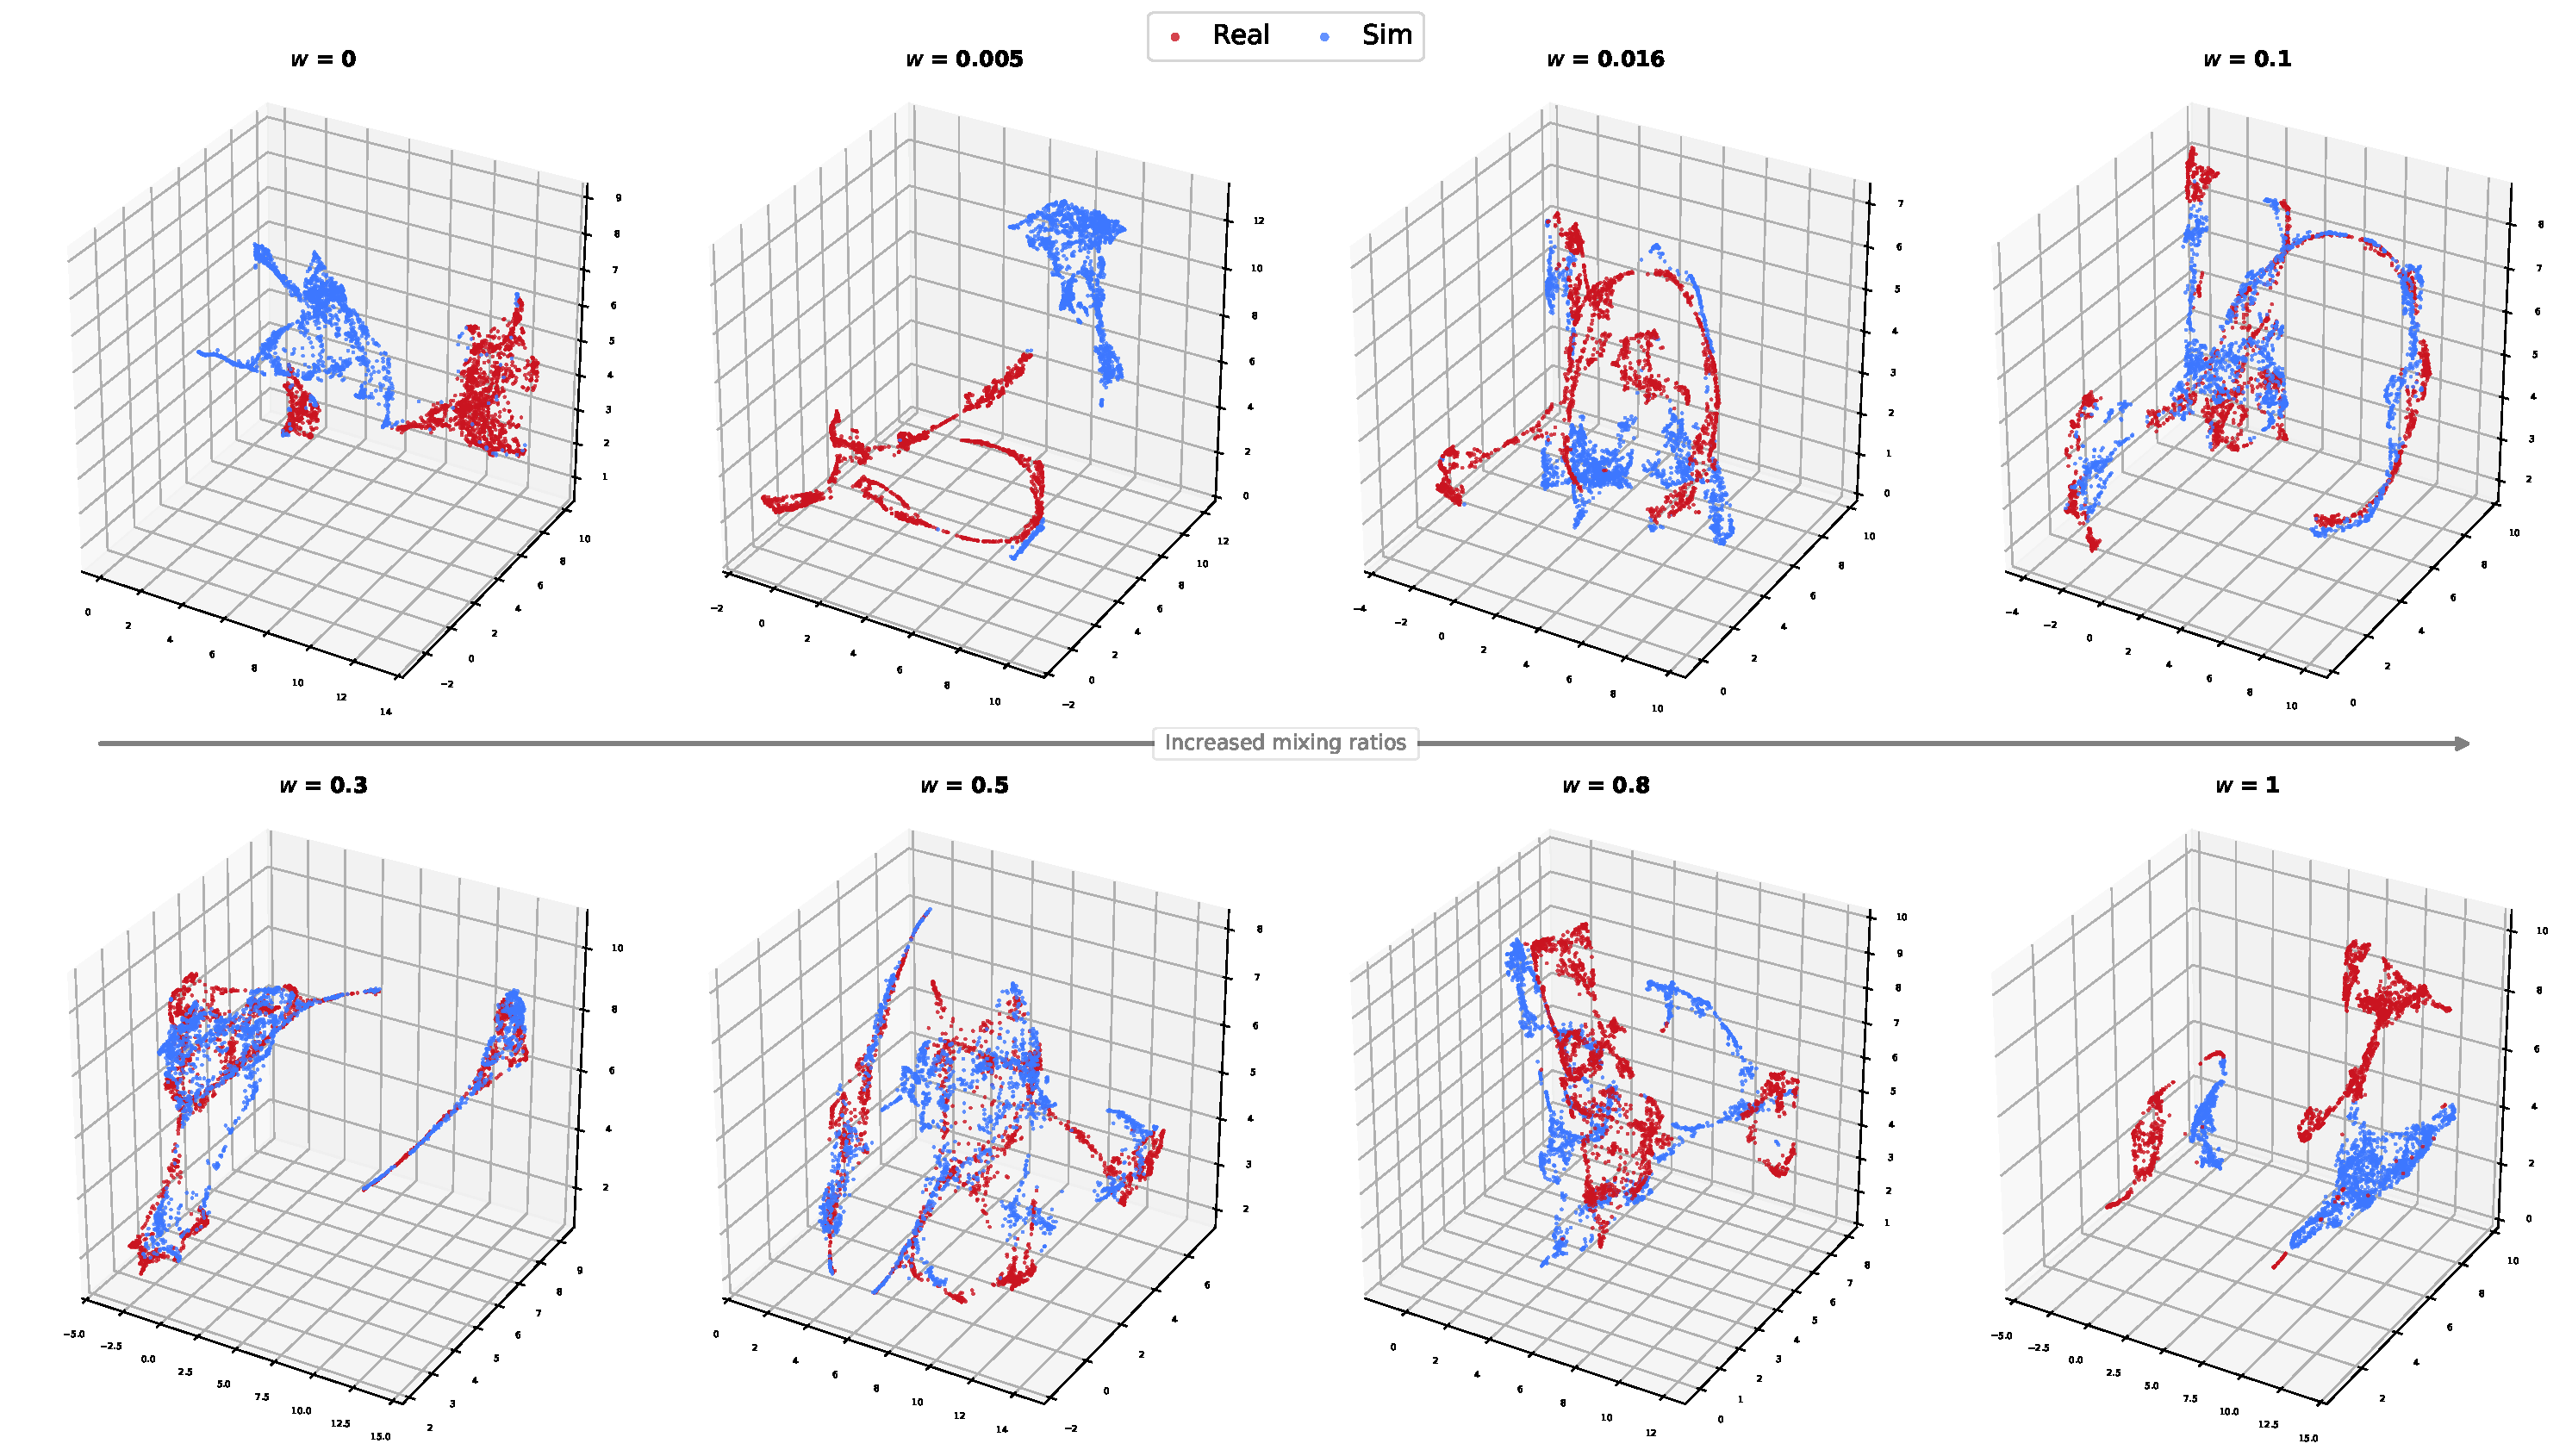
\includegraphics[width=\textwidth, height=2.8in]{asset/mugcleanup_trans_feat.pdf}
        \caption{\texttt{MugCleanup}.}
    \end{subfigure}}
    \vfill
    \resizebox{0.98\linewidth}{!}{
    \begin{subfigure}{\linewidth}
        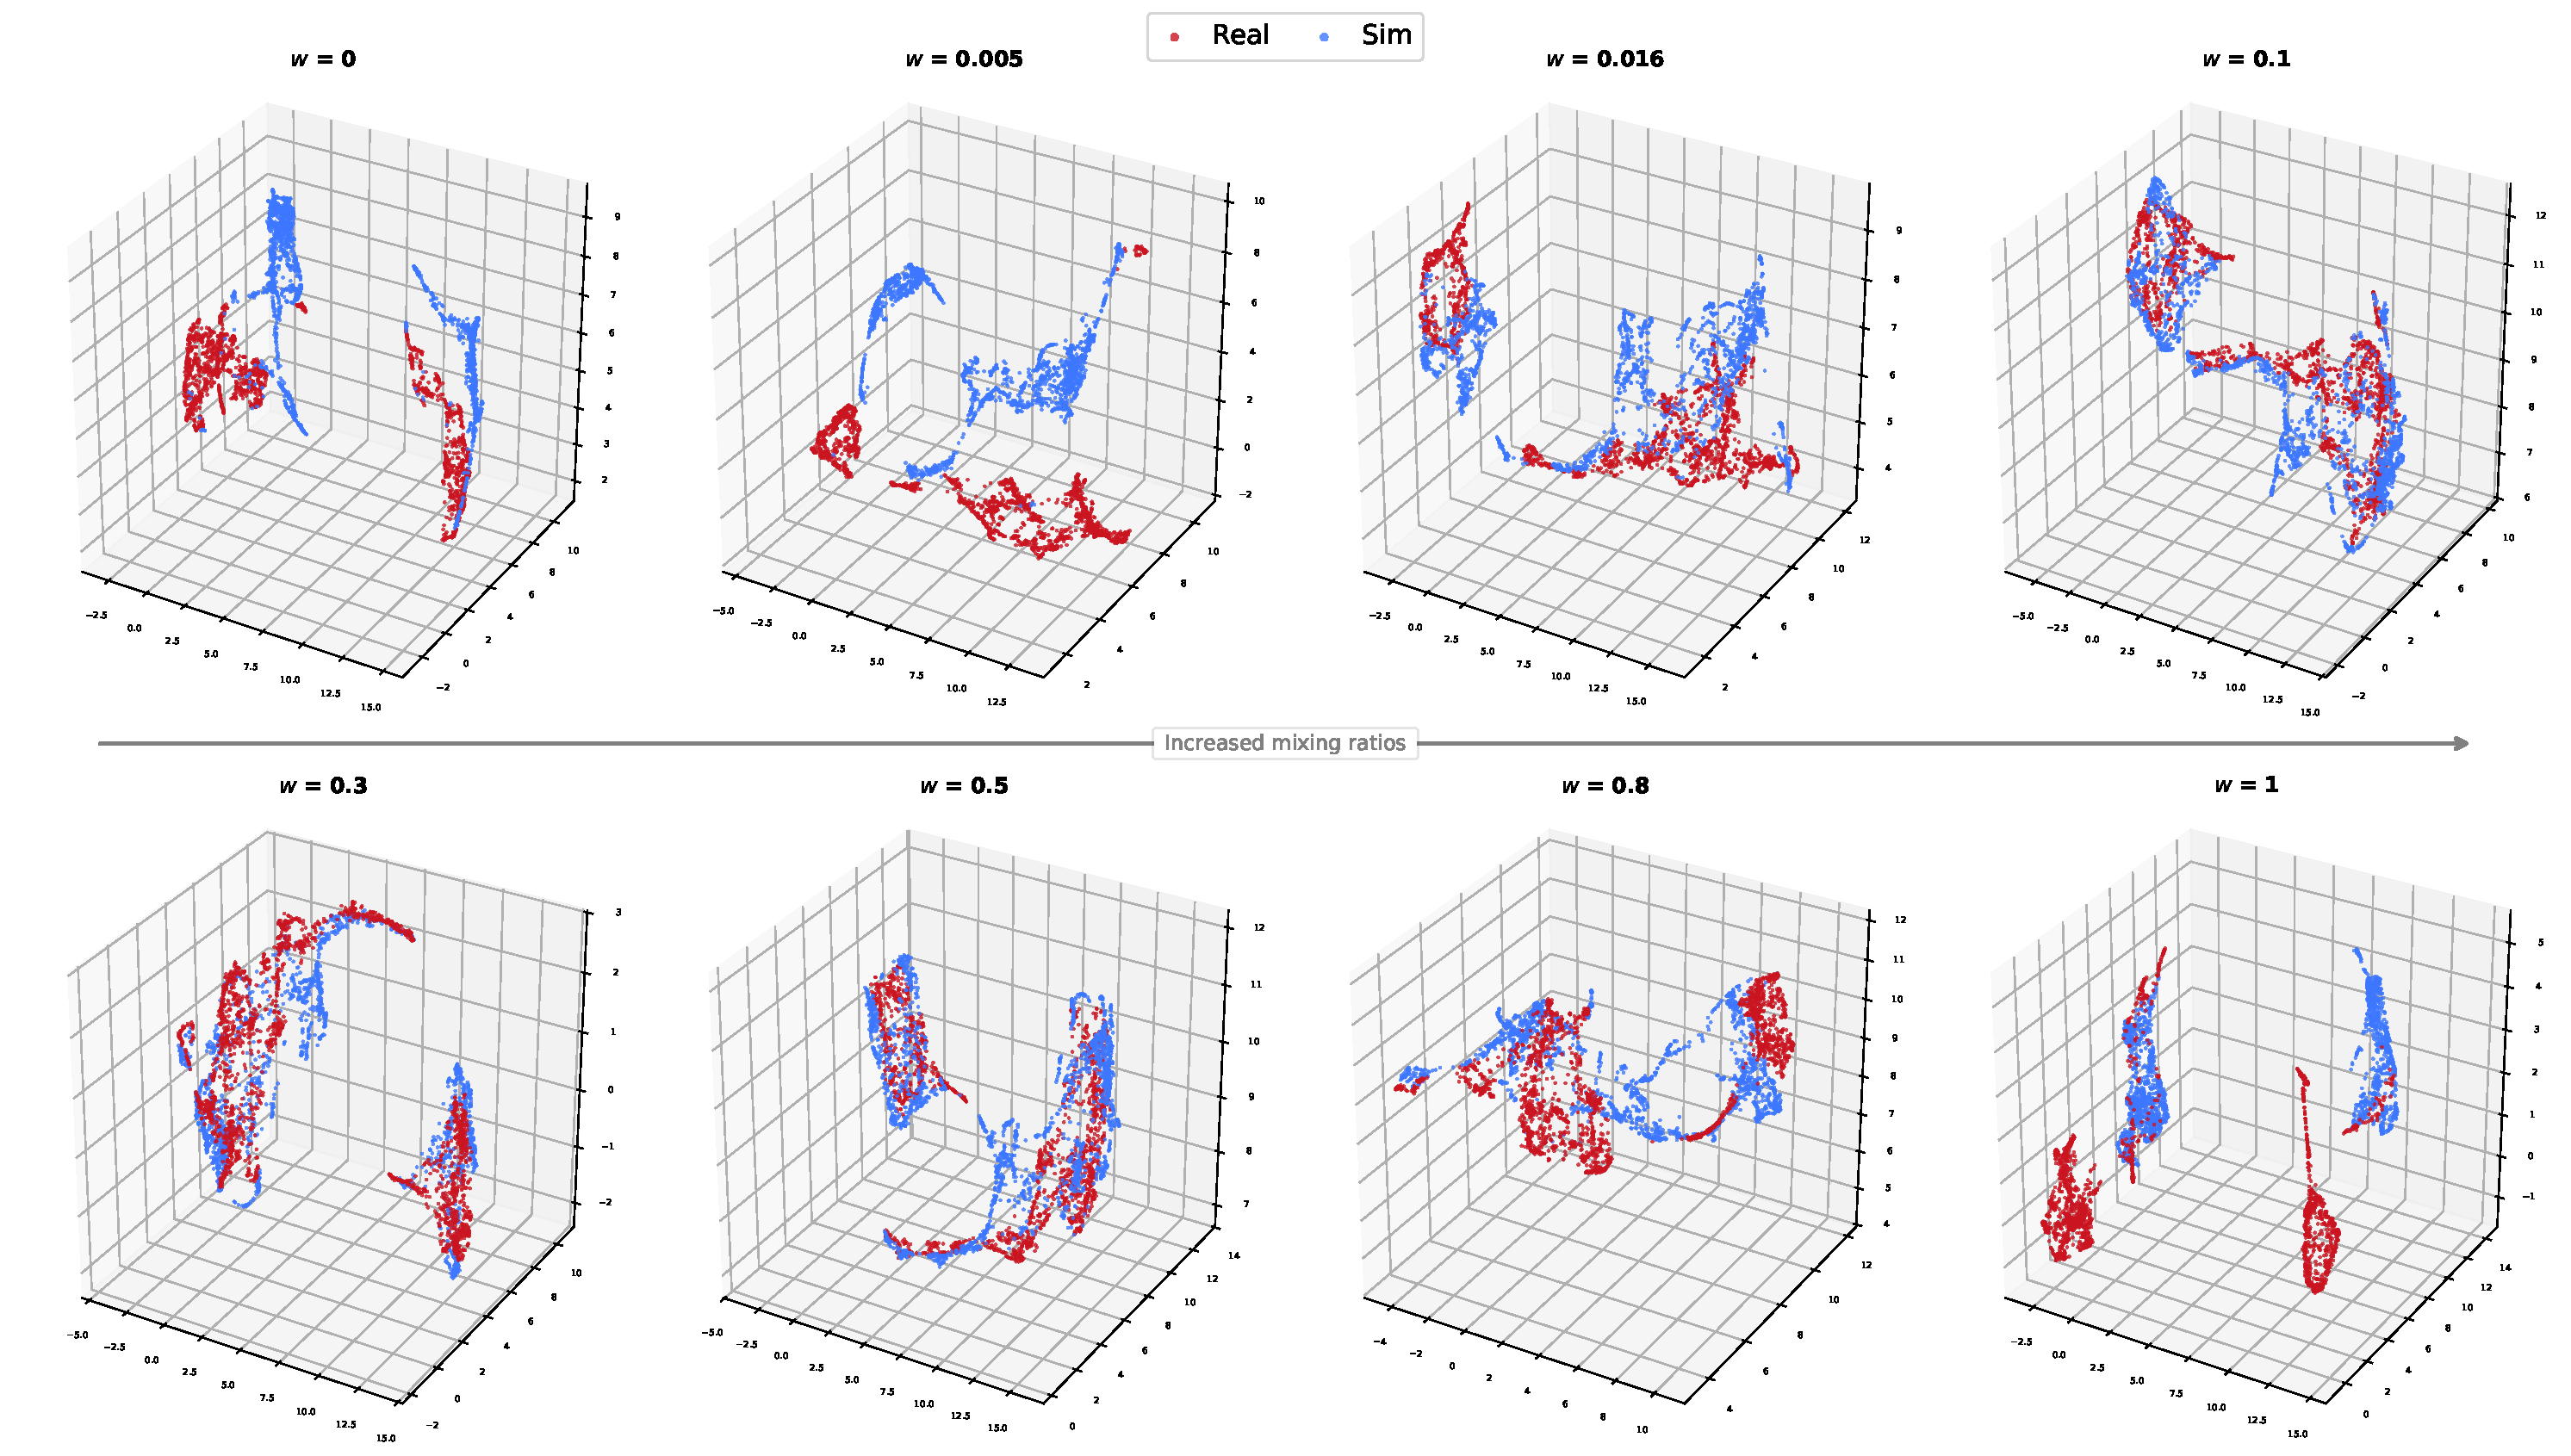
\includegraphics[width=\textwidth, height=2.8in]{asset/mughang_trans_feat.pdf}
        \caption{\texttt{MugHang}.}
    \end{subfigure}}
    \caption{\textbf{More UMAP visualizations of the deeper layer representations.} }
    \vspace{-10pt}
    \label{fig: more feature vis2}
\end{figure}




% You can have as much text here as you want. The main body must be at most $8$
% pages long. For the final version, one more page can be added. If you want, you
% can use an appendix like this one.

% The $\mathtt{\backslash onecolumn}$ command above can be kept in place if you
% prefer a one-column appendix, or can be removed if you prefer a two-column
% appendix.  Apart from this possible change, the style (font size, spacing,
% margins, page numbering, etc.) should be kept the same as the main body.
%%%%%%%%%%%%%%%%%%%%%%%%%%%%%%%%%%%%%%%%%%%%%%%%%%%%%%%%%%%%%%%%%%%%%%%%%%%%%%%
%%%%%%%%%%%%%%%%%%%%%%%%%%%%%%%%%%%%%%%%%%%%%%%%%%%%%%%%%%%%%%%%%%%%%%%%%%%%%%%